\documentclass[11pt, a4paper]{report}
\pagestyle{headings}
\usepackage[pagestyles]{titlesec}
\usepackage{lipsum}
\usepackage[ngerman]{babel}
\usepackage[utf8]{inputenc}
\usepackage[T1]{fontenc}
\usepackage{graphicx}
\usepackage{geometry}
\usepackage{caption}
\usepackage[hidelinks]{hyperref}
\usepackage{listingsutf8}
\usepackage{float}
\usepackage{setspace}
\usepackage{xcolor}
\usepackage{amsmath}
\usepackage{amssymb}
\usepackage{csquotes}
\usepackage[backend=biber, style=authoryear]{biblatex}
\addbibresource{sources.bib}
\setlength{\bibitemsep}{1em}
\DeclareLabeldate{
    \field{date}
    \field{eventdate}
    \field{origdate}
    \literal{nodate}
}

% Add substitutes for umlauts
\lstset{
    inputencoding=utf8,
    extendedchars=true,
    literate=%
    {Ä}{{\"A}}1
    {Ö}{{\"O}}1
    {Ü}{{\"U}}1
    {ä}{{\"a}}1
    {ö}{{\"o}}1
    {ü}{{\"u}}1
}

% Define Solidity as a language for listings because it is not supported by default
\lstdefinelanguage{Solidity}{
  keywords={address, bool, string, uint, mapping, contract, function, modifier, event, require, assert, bytes},
  keywordstyle=\color{blue}\bfseries,
  identifierstyle=\color{black},
  sensitive=false,
  comment=[l]{//},
  morecomment=[s]{/*}{*/},
  commentstyle=\color{gray}\ttfamily,
  stringstyle=\color{teal}\ttfamily,
  morestring=[b]',
  morestring=[b]"
}

% Define the Solidity style for listings
\lstset{
  language=Solidity,
  basicstyle=\small\ttfamily,
  breaklines=true,
  showstringspaces=false,
  numbers=left,
  numberstyle=\tiny\color{gray},
  numbersep=5pt,
  tabsize=2,
  frame=lines,
  showtabs=false,
  showspaces=false,
  extendedchars=true,
  inputencoding=utf8,
  captionpos=b
}

% \makeatletter
% \def\thickhrulefill{\leavevmode \leaders \hrule height 1ex \hfill \kern \z@}
% \def\@makechapterhead#1{%
%   \vspace*{10\p@}%
%   {\parindent \z@ 
%     {\raggedleft \reset@font
%       \fontsize{15ex}{15ex}\selectfont %Problème avec les substitutions...
%       \bfseries\thechapter\par\nobreak}%
%     \par\nobreak
%     \interlinepenalty\@M
%     {\raggedright \Huge \bfseries #1}%
%     \par\nobreak
%     \hrulefill
%     \par\nobreak
%     \vskip 100\p@
%   }}
% \def\@makeschapterhead#1{%
%   \vspace*{10\p@}%
%   {\parindent \z@ 
%     {\raggedleft \reset@font
%       \fontsize{15ex}{15ex}\selectfont %Problème avec les substitutions...
%       \bfseries\vphantom{\thechapter}\par\nobreak}%
%     \par\nobreak
%     \interlinepenalty\@M
%     {\raggedright \Huge \bfseries #1}%
%     \par\nobreak
%     \hrulefill
%     \par\nobreak
%     \vskip 100\p@
%   }}
  
%%%%%%%%%%%%%%%%%%%%%%%%%%%%%% NOTES %%%%%%%%%%%%%%%%%%%%%%%%%%%%%%

% - Keep the standard LaTeX font?
%     NOTE: when using Tahoma font, you have to compile this with XeLaTeX (xelatex) or 
%    LuaLaTeX (lualatex) instead of regular LaTeX.
% - Why Kademlia and not Chord? Kademlia:
% Efficient Asymmetric Routing: Kademlia uses XOR metric-based routing to perform lookups. It's efficient and has an asymmetric routing mechanism, allowing for faster lookups in certain scenarios, especially when there are geographical considerations or when the system has a high rate of node churn.
% Resilience to Churn: Kademlia tends to handle high rates of node joining and leaving more gracefully than some other DHTs, making it more suitable for dynamic networks.
% Decentralization and Redundancy: Kademlia offers decentralized storage and redundancy, ensuring that data is stored in multiple nodes for fault tolerance.
% #TODO: Change signature to a nicer version!

%%%%%%%%%%%%%%%%%%%%%%%%%%%%%%%%%%%%%%%%%%%%%%%%%%%%%%%%%%%%%%%%%%%

\begin{document}
    % Custom title page
    \begin{titlepage}
        \begin{center}
            
            \vspace*{1cm}
            \LARGE
            \textbf{Bachelorarbeit}\\

            \Large
            \bigbreak
            im Studiengang \\
            Wirtschaftsinformatik und digitale Medien\\

            \vspace*{1cm}
            \LARGE
            \textbf{Ein sicheres Peer-to-Peer-Instant-Messaging-Protokoll unter
            Berücksichtigung von Blockchain-Technologie}\\
            
            \large
            \vspace*{1cm}
            vorgelegt von \\
            \vspace*{0.5cm}
            \textbf{Nicole Sauer} \\
            \vspace*{1cm}

            
\includegraphics[width=0.2\linewidth]{images/hdm_logo.png} \\

            \vspace*{0.5cm}
            an der Hochschule der Medien Stuttgart \\
            am 29.01.2024 \\
            zur Erlangung des akademischen Grades eines \\
            \textbf{Bachelor of Science}\\
            \vspace*{1.5cm}
            \large 
            \begin{tabular}{ll}
                Erstprüfer & Prof. Dr. Peter Thies \\
                Zweitprüfer & Prof. Dr. Stephan Wilczek \\
            \end{tabular} \\
        \end{center}
    \end{titlepage}
    
    % Change vertical spacing to 1.5 for the rest of the document
    \onehalfspacing

    %%%%%%%%%%%%%%%%%%%%%%%% BEGIN: ToC, LoF, Abstract DE/ENG, Ehrenw. Erkl. %%%%%%%%%%%%%%%%%%%%%%%%
    %\chapter*{Ehrenwörtliche Erklärung}

Hiermit versichere ich, Nicole Sauer, ehrenwörtlich, dass ich die vorliegende 
Bachelorarbeit mit dem Titel: \enquote{Ein sicheres Peer-to-Peer-Instant-Messaging-Protokoll unter
Berücksichtigung von Blockchain-Technologie} selbstständig und ohne fremde Hilfe verfasst und keine anderen 
als die angegebenen Hilfsmittel benutzt habe. Die Stellen der Arbeit, die dem Wortlaut oder dem Sinn nach 
anderen Werken entnommen wurden, sind in jedem Fall unter Angabe der Quelle kenntlich gemacht. Ebenso sind alle
Stellen, die mit Hilfe eines KI-basierten Schreibwerkzeugs erstellt oder überarbeitet wurden, kenntlich
gemacht. Die Arbeit ist noch nicht veröffentlicht oder in anderer Form als Prüfungsleistung vorgelegt worden. \\
\\
Ich habe die Bedeutung der ehrenwörtlichen Versicherung und die prüfungsrechtlichen Folgen 
(§ 24 Abs. 2 Bachelor-SPO), der HdM einer unrichtigen oder unvollständigen 
ehrenwörtlichen Versicherung zur Kenntnis genommen.
\\
\\

\noindent\begin{tabular}{ll}
    Leutenbach, den 29.01.2024 & 
\includegraphics[width=0.25\linewidth]{images/signature2.jpg} \\
    \makebox[6cm]{\hrulefill} & \makebox[6cm]{\hrulefill}\\
    Ort, Datum & Unterschrift\\
\end{tabular}

    \tableofcontents
    %\listoffigures
    %\lstlistoflistings
    %\chapter*{Kurzfassung}

Diese Bachelorarbeit präsentiert die Entwicklungsarbeit an einem innovativen Peer-to-Peer-Instant-Messaging-Protokoll, das auf einer Kombination von Kademlia und Interactive Connectivity Establishment (ICE) basiert. Der Fokus liegt auf der Schaffung eines dezentralen, robusten Peer-to-Peer Kommunikationsprotokolls, das unabhängig von zentralen Servern agiert.

Die Authentifizierung der Teilnehmer erfolgt über öffentliche Schlüssel, die sicher in der Ethereum Blockchain hinterlegt sind. Diese Blockchain-basierte Authentifizierung gewährleistet eine vertrauenswürdige Identitätsüberprüfung, wobei die dezentrale Natur von Ethereum eine hohe Sicherheit und Manipulationssicherheit bietet.

Ein zentraler Beitrag dieser Arbeit ist die Integration von Kademlia, einem verteilten Peer-to-Peer Routing-Algorithmus, und ICE, einem Mechanismus zur Überquerung von Netzwerkgrenzen. Diese Kombination ermöglicht eine effiziente und zuverlässige P2P-Kommunikation, wodurch die Abhängigkeit von zentralen Servern minimiert wird. Die Implementierung wurde darauf ausgerichtet, eine hohe Skalierbarkeit und Robustheit des Systems sicherzustellen.

Die präsentierte Lösung bietet nicht nur eine sichere Peer-to-Peer Kommunikationsumgebung, sondern betont auch die Bedeutung der Blockchain-Technologie für die Authentifizierung in dezentralen Systemen. Das entwickelte Protokoll demonstriert, wie eine Kombination von Ethereum, Kademlia und ICE die Grundlage für eine vertrauenswürdige und effiziente Peer-to-Peer-Instant-Messaging-Infrastruktur schaffen kann.
    %\chapter*{Abstract}

% #TODO: Abstract schreiben

This bachelor's thesis introduces the development of an innovative Peer-to-Peer Instant Messaging protocol, leveraging a combination of Kademlia and Interactive Connectivity Establishment (ICE). The primary focus lies in creating a decentralized, robust Peer-to-Peer communication protocol that operates independently of central servers.

Participant authentication is achieved through public keys securely stored in the Ethereum blockchain. This blockchain-based authentication ensures a trustworthy identity verification process, with Ethereum's decentralized nature providing high security and tamper resistance.

A significant contribution of this work is the integration of Kademlia, a distributed Peer-to-Peer routing algorithm, and ICE, a mechanism for traversing network boundaries. This combination enables efficient and reliable P2P communication, minimizing reliance on central servers. The implementation is designed for high scalability and system robustness.

The presented solution not only offers a secure Peer-to-Peer communication environment but also underscores the importance of blockchain technology for authentication in decentralized systems. The developed protocol demonstrates how a combination of Ethereum, Kademlia, and ICE can form the foundation for a trusted and efficient Peer-to-Peer Instant Messaging infrastructure.
    %%%%%%%%%%%%%%%%%%%%%%%%% END: ToC, LoF, Abstract DE/ENG, Ehrenw. Erkl. %%%%%%%%%%%%%%%%%%%%%%%%%


    %%%%%%%%%%%%%%%%%%%%%%%%%%%%%%%%%%%% BEGIN: Numbered Chapters %%%%%%%%%%%%%%%%%%%%%%%%%%%%%%%%%%%
    \chapter{Einleitung}
\label{chap:einleitung}

% Motivation aufzeigen: Diese Bachelorarbeit setzt sich mit der Herausforderung auseinander, ein Peer-to-Peer-Instant-Messaging-Protokoll zu entwickeln, das nicht nur die Privatsphäre seiner Benutzer schützt, sondern auch durch die Integration von Blockchain-Technologie die Integrität und Authentizität der Kommunikation gewährleisten kann.

In den letzten Jahren hat sich die digitale Kommunikation signifikant gewandelt. 2013 war das Short Message System (SMS) noch dominierend, doch in den darauf folgenden Jahren verlagerte sich der Fokus deutlich hin zum Mobile-Instant-Messaging. Die Nutzung von Instant-Messaging unter der deutschen Bevölkerung stieg von etwa 24\% im Jahr 2013 auf beeindruckende 73\% im Jahr 2017 \parencite{Hedda_digiKommunikationVeraendert}. Die Gründe für diesen Wandel sind vielfältig. Instant-Messaging ist in der Regel kostenlos, schnell und einfach zu bedienen. Darüber hinaus bietet es viele nützliche Funktionen wie Gruppenchats, Sprach- und Videoanrufe, Dateiübertragung und vieles mehr. Instant-Messaging ist zu einem wichtigen Bestandteil unseres täglichen Lebens geworden. Es ist ein wesentlicher Bestandteil der Kommunikation zwischen Freunden und Familie, aber auch zwischen Kollegen und Geschäftspartnern. 

Aber Instant-Messaging ist nicht gleich Instant-Messaging. Es gibt verschiedene Arten von Instant-Messaging-Diensten, die sich in ihrer Funktionsweise und ihren Eigenschaften unterscheiden. Die bekanntesten sind zentralisierte und dezentrale Instant-Messaging-Dienste. Zentralisierte Dienste werden von einem zentralen Server verwaltet, der die Kommunikation zwischen den Benutzern vermittelt. Dezentrale Dienste hingegen nutzen eine Peer-to-Peer-Infrastruktur, bei der die Kommunikation direkt zwischen den Benutzern stattfindet. 

Zentralisierte Dienste sind in der Regel einfach zu bedienen und bieten eine gute Benutzererfahrung. Sie sind jedoch anfällig für Sicherheitsbedrohungen, da die Kommunikation über einen zentralen Server vermittelt wird. Sollte dieser Server kompromittiert werden, könnte die Kommunikation der Benutzer abgefangen oder manipuliert werden. Darüber hinaus könnten die Betreiber des Dienstes die Kommunikation ihrer Benutzer überwachen und speichern. Dies stellt ein großes Problem für die Privatsphäre der Benutzer dar.

Dezentrale Dienste hingegen haben das Potenzial mehr Sicherheit und Privatsphäre für ihre Nutzer zu bieten, da die Kommunikation direkt zwischen den Benutzern stattfindet. Es gibt keinen zentralen Server, der angegriffen werden könnte. Darüber hinaus können die Betreiber des Dienstes die Kommunikation nicht überwachen, da sie nicht an der Kommunikation beteiligt sind. Dezentrale Dienste sind jedoch in der Regel komplexer und schwieriger zu bedienen als zentralisierte Dienste. Und auch sie sind nicht perfekt. Auch in dezentralen Diensten können Sicherheitslücken auftreten, die die Sicherheit und Privatsphäre der Benutzer gefährden.


Durch die im Jahr 2013 von Edward Snowden veröffentlichten Dokumente wurde deutlich, dass die Kommunikation von Millionen von Menschen von Geheimdiensten überwacht wurde \parencite{greenwald_NSA}. Dadurch rückten die Themen Sicherheit und Privatsphäre in den Fokus der Öffentlichkeit. Durch diese Enthüllungen entstand zum Beispiel das Peer-to-Peer-Instant-Messaging-Protokoll \textit{Tox}. Es wurde von einer Gruppe von Entwicklern ins Leben gerufen, die sich zum Ziel gesetzt haben, ein sicheres und leicht zu bedienendes Instant-Messaging-Protokoll zu entwickeln, das die Privatsphäre seiner Benutzer schützt \parencite{tox_about}. Die Entwicklung eines solchen Instant-Messaging-Protokolls ist jedoch nicht leicht. Es müssen viele Aspekte beachtet werden, die in zentralisierten Protokollen nicht vorhanden sind und die die Komplexität des Protokolls erhöhen. Im Verlauf dieser Bachelorarbeit werden verschiedene Aspekte der Peer-to-Peer-Kommunikation, einschließlich Sicherheit, Effizienz und Benutzerfreundlichkeit, beleuchtet. Dabei werden auch bereits verfügbare Protokolle betrachtet, um eine Grundlage für die Entwicklung eines eigenen Protokolls zu schaffen. Darüber hinaus hat die Blockchain das Potenzial, die Integrität und Authentizität von Daten und Dokumenten in Instant Messaging-Plattformen sicherzustellen, weshalb auch diese Technologie in dieser Arbeit betrachtet wird.

Diese Bachelorarbeit konzentriert sich auf die Herausforderung, ein Peer-to-Peer-Instant-Messaging-Protokoll zu konzipieren. Dabei liegt der Fokus nicht nur darauf, die Privatsphäre der Nutzer zu bewahren, sondern auch die Integrität und Authentizität der Kommunikation durch die Integration von Blockchain-Technologie zu gewährleisten. Das Hauptziel besteht darin, einen Prototypen für ein derartiges Protokoll zu entwickeln, der durch den Einsatz von Blockchain-Technologie die Sicherheit der Kommunikation verbessern soll. Der Prototyp soll dabei als Demonstrationsmittel dienen und die praktische Umsetzbarkeit eines solchen Protokolls verdeutlichen.

    \chapter{Grundlagen}

\section{Instant Messaging}
% Was ist Instant Messaging?
% Wofür wird es verwendet?
% Welche Anwendungen gibt es? (WhatsApp, Signal, Telegram, Threema, etc.) -> die meisten sind zentralisiert
% Welche Probleme gibt es bei zentralisierten Anwendungen?
% Client-Server-Architektur und Peer to Peer als Überleitung zur nächsten Sektion verwenden


Instant Messaging bezeichnet eine Form der Kommunikation, bei der Nachrichten in Echtzeit zwischen zwei oder mehreren Personen über das Internet ausgetauscht werden können \Parencite[S. 69]{nist_mobileDeviceForensics}. Diese Form der digitalen Kommunikation ermöglicht es Nutzern, sofortige Nachrichten, Bilder und andere Mediendateien auszutauschen. Instant Messaging-Dienste umfassen eine Vielzahl von Plattformen und Anwendungen, die es Benutzern ermöglichen, miteinander zu kommunizieren, sei es eins zu eins oder in Gruppenchats. Instant-Messaging-Dienste reichen von plattformübergreifenden Anwendungen wie \textit{WhatsApp}, \textit{Signal} und \textit{Telegram} bis hin zu spezialisierten Unternehmenslösungen wie \textit{Slack} oder \textit{Microsoft Teams}. Die Vielfalt an Funktionen in Instant-Messaging-Plattformen ist groß. Neben einfachen Textnachrichten können Benutzer zum Beispiel mit der App \textit{WhatsApp} Emojis, Aufkleber, GIFs und Sprachnachrichten teilen, was die Kommunikation dynamisch und ausdrucksstark gestaltet \Parencite{whatsapp_funktionen}. Gruppenchats ermöglichen es mehreren Personen, in einer einzigen Unterhaltung zusammenzukommen, was die Zusammenarbeit, soziale Interaktion und Informationsverbreitung erleichtert.
Sicherheit und Datenschutz sind in der Welt des Instant Messaging von entscheidender Bedeutung. Verschlüsselungstechnologien werden verwendet, um die Vertraulichkeit der Nachrichten zu gewährleisten und die Privatsphäre der Nutzer zu schützen. Die Authentifizierung von Benutzern, End-to-End-Verschlüsselung und andere Sicherheitsmechanismen sind unerlässlich, um die Integrität der Kommunikation zu gewährleisten.

Instant Messaging-Anwendungen können auf verschiedene Arten strukturiert sein, wobei zwei Hauptansätze hervorstechen: die Client-Server-Architektur und das Peer-to-Peer-Modell.
Die Client-Server-Architektur ist bei vielen gängigen Instant Messaging-Diensten verbreitet. Hierbei fungiert ein zentraler Server als Vermittler zwischen den Benutzergeräten. Die Nachrichten werden von den Clients (den Benutzergeräten) an den Server gesendet, der sie dann an die Empfänger weiterleitet. Dieser Ansatz bietet eine einfache Verwaltung der Kommunikation, zentralisierte Datenverwaltung und ermöglicht Dienstleistungen wie das Offline-Speichern von Nachrichten.
Im Gegensatz dazu basiert das Peer-to-Peer-Modell (kurz: P2P) auf direkten Verbindungen zwischen den Benutzergeräten ohne die Notwendigkeit eines zentralen Servers. Jedes Gerät agiert sowohl als Client als auch als Server, wodurch die Kommunikation direkt zwischen den Teilnehmern stattfindet. Diese Struktur bietet potenzielle Vorteile in Bezug auf Datenschutz, da die Nachrichten nicht über einen zentralen Server geleitet werden müssen.
Beide Ansätze haben ihre eigenen Vor- und Nachteile. Die Client-Server-Architektur ermöglicht eine einfachere Verwaltung und Zuverlässigkeit, birgt jedoch potenzielle Datenschutzrisiken, da Daten zentralisiert gespeichert werden. Auf der anderen Seite bietet das Peer-to-Peer-Modell potenziell mehr Privatsphäre und Sicherheit, aber es könnte Schwierigkeiten bei der Skalierbarkeit und Verlässlichkeit geben, da es keine zentrale Instanz gibt, die die Kommunikation steuert. Die Wahl zwischen diesen Architekturen hängt von den spezifischen Anforderungen, Sicherheitsbedenken und dem Nutzungskontext der Instant Messaging-Anwendung ab.



\section{Blockchain-Technologie}
Die Blockchain-Technologie ist... . Blockchains sind auch bekannt als Distributed Ledger 
Technology (DLT) und das sind auch nur verteilte Datenbanken. Die Blockchain ist eine
spezielle Form der DLT. Die Blockchain ist eine Kette von Blöcken, die jeweils einen
Hash des vorherigen Blocks enthalten. Die Blockchain ist eine dezentrale Datenbank, die
von allen Teilnehmern des Netzwerks verwaltet wird.

Proof of Work und Proof of Stake sind zwei verschiedene Konsensmechanismen, die verwendet
werden, um die Blockchain zu validieren. Proof of Work ist der Konsensmechanismus, der
von Bitcoin verwendet wird. Proof of Stake ist der Konsensmechanismus, der von Ethereum (2.0)
verwendet wird.

\subsection{Ethereum}
\label{sec:ethereum_basics}

Ethereum ist eine der führenden Blockchain-Plattformen und wurde 2015 von Vitalik Buterin, Gavin Wood und anderen entwickelt. Im Gegensatz zu Bitcoin, das hauptsächlich als digitale Währung fungiert, ermöglicht Ethereum die Ausführung von Smart Contracts und die Entwicklung von dezentralen Anwendungen (engl. \textit{decentralized Applications}, kurz \textit{DApps}) \Parencites[S. 720]{Sorge_BitcoinZahlungsmittelDerZukunft}[S. 1-2]{Perez_SmartContractVulnerabilities}. Bis 2022 wurde als Konsensmechanismus Proof-of-Work verwendet, der jedoch 2022 durch Proof-of-Stake ersetzt wurde. Seitdem existieren zwei Versionen von Ethereum: \textit{Ethereum Classic} und \textit{Ethereum 2.0}. Ethereum Classic verwendet Proof-of-Work, während Ethereum 2.0 Proof-of-Stake verwendet \Parencite{EthereumClassic_ResearcherFAQs}.

Ether (ETH) ist die native Kryptowährung von Ethereum und wird für Transaktionen innerhalb des Netzwerks verwendet. Es dient auch als Anreiz für diejenigen, die an der Sicherung des Netzwerks durch Mining (bei PoW) oder Validierung (bei PoS) von Transaktionen beteiligt sind \parencite[S. 320-321]{Antonopoulos_MasteringEthereum}. Die Flexibilität von Ethereum und seine Fähigkeit, innovative Lösungen zu unterstützen, haben es zu einer der wichtigsten Plattformen in der Blockchain-Welt gemacht.

\subsection{Smart Contracts}
\label{subsection:smart_contracts}
% Smart Contracts werden per RPC aufgerufen.


Ein Smart Contract (zu Deutsch: \textit{intelligenter Vertrag}) ist im Grunde genommen ein selbstausführender Vertrag, der automatisch Aktionen auslöst, wenn bestimmte Bedingungen erfüllt sind \Parencite[S. 1-2]{Perez_SmartContractVulnerabilities}. Die Bezeichnung \textit{Smart Contract} ist eigentlich eine Fehlbezeichnung, da es sich weder um einen Vertrag im rechtlichen Sinne, noch um einen \textit{intelligenten} Vertrag handelt, doch der Begriff hat sich in der Blockchain-Community etabliert und wird deshalb weiterhin verwendet. Ein Lesezugriff auf einen Smart Contract ist kostenlos, ein Schreibzugriff hingegen kostet Geld, da die Transaktion in der Blockchain gespeichert werden muss. Dieses Geld wird als \textit{Gas} bezeichnet und ist eine Art Gebühr, die gezahlt werden muss, um die Rechenleistung des Netzwerks zu nutzen \Parencite[S. 127]{Antonopoulos_MasteringEthereum}. Um Gas zu erhalten, muss der Nutzer Ether eintauschen, die Währung der Ethereum-Blockchain.
Für das Protokoll dieser Arbeit wurden sowohl Lese- als auch Schreibzugriffe auf Smart Contracts implementiert (siehe Kapitel \ref{chap:entwurf_und_architektur} \textit{\nameref{chap:entwurf_und_architektur}}).

Die Plattform verwendet die objektorientierte Programmiersprache \textit{Solidity}, die speziell für Smart Contracts entwickelt wurde und stark an JavaScript angelehnt ist. Entwickler können mithilfe von Solidity Smart Contracts erstellen, die dann in der Ethereum-Blockchain ausgeführt werden und von jedem Teilnehmer des Netzwerks aufgerufen werden können \Parencite[S. 127-133]{Antonopoulos_MasteringEthereum}.


\section{Peer-to-Peer-Technologie}
\label{subsec:peer_to_peer_technologie}
% #TODO: Funktion des Kademlia Protokolls nennen und erklären (vielleicht in Grundlagen)
% Im Kademlia-Protokoll sind vier Funktionen definiert, die für die Suche nach
% Knoten und Werten verwendet werden. Diese Funktionen sind \texttt{FIND\_NODE},
% \texttt{FIND\_VALUE}, \texttt{PING} und \texttt{STORE}. Die Funktionen
% \texttt{FIND\_NODE} und \texttt{FIND\_VALUE} werden verwendet, um nach Knoten
% oder Werten zu suchen. Die Funktion \texttt{PING} wird verwendet, um die
% Erreichbarkeit eines Knotens zu überprüfen. Die Funktion \texttt{STORE} wird
% verwendet, um einen Wert in einem Knoten zu speichern.

Peer-to-Peer-Technologien können in zwei Kategorien unterteilt werden: Peer-to-Peer-Anwendungen und Peer-to-Peer-Infrastrukturen. Die Kategorie der Peer-to-Peer-Anwen-\\dungen umfasst den Dienst der Inhaltsverteilung, bei dem die Teilnehmer Inhalte wie Musik, Videos oder andere Dateien direkt untereinander austauschen \Parencite[730-731]{Khatibi_StructuredUnstructuredP2P}. 

Daher werden viele Peer-to-Peer schnell mit Filesharing in Verbindung bringen, da diese Technologie in der Vergangenheit vor allem dafür genutzt wurde. Das bekannteste Beispiel ist das Filesharing-Netzwerk \textit{Napster}, das 1999 von Shawn \enquote{Napster} Fanning entwickelt wurde. \textit{Napster} war das erste weit verbreitete Filesharing-Netzwerk, das auf Peer-to-Peer-Technologie basierte. Es ermöglichte den Austausch von Musikdateien zwischen den Teilnehmern. Die Musikdateien wurden dabei auf den Computern der Teilnehmer gespeichert und konnten von anderen Teilnehmern heruntergeladen werden. Da diese Art des Datenaustauschs oftmals illegal war, wurde Napster 2001 aufgrund von Urheberrechtsverletzungen abgeschaltet \parencite[S. 55-57]{Mahlmann_P2PNetzwerke}.

Die Peer-to-Peer-Infrastruktur umfasst die Peer-to-Peer-Netzwerke, die für die Kommunikation zwischen den Teilnehmern verwendet werden \parencite[S. 730-731]{Khatibi_StructuredUnstructuredP2P}. Diese Arbeit konzentriert sich auf die Peer-to-Peer-Infrastruktur, die die Kommunikation zwischen den Teilnehmern ermöglichen soll.

Im Instant-Messaging-Bereich repräsentiert das Peer-to-Peer-Modell eine dezentrale Struktur, die dabei hilft, die Kommunikation zwischen den Teilnehmern zu ermöglichen. Im Gegensatz zum Client-Server-Ansatz, bei dem ein zentraler Server die Kommunikation zwischen den Teilnehmern steuert, ermöglicht das Peer-to-Peer-Netzwerk direkte Kommunikation zwischen den Teilnehmern. Beide Modelle bringen Vor- und Nachteile mit sich. Während das Client-Server-Modell eine zentrale Instanz erfordert, um die Kommunikation zu verwalten, ist das Peer-to-Peer-Netzwerk dezentralisiert und benötigt keine solche Instanz. Die Implementierung und Wartung eines Client-Server-Modells gestalten sich einfacher im Vergleich zu einem komplexeren und aufwendigeren Peer-to-Peer-Netzwerk. Das Client-Server-Modell ist weniger flexibel, da es von einer zentralen Instanz abhängt, während das Peer-to-Peer-Netzwerk aufgrund des Fehlens dieser Instanz flexibler ist. Skalierbarkeit ist ebenfalls ein Unterschied: Das Client-Server-Modell ist durch die Kapazität des Servers begrenzt, während das Peer-to-Peer-Netzwerk auf die Kapazität der Teilnehmer zurückgreift, was seine Skalierbarkeit verbessert. In Bezug auf Sicherheit ist das Client-Server-Modell weniger robust, da es auf eine zentrale Instanz angewiesen ist, während das Peer-to-Peer-Netzwerk, das ohne solche Abhängigkeit auskommt, als sicherer gilt \parencite[S. 6-8]{Mahlmann_P2PNetzwerke}.


\subsection{Typen von Peer-to-Peer-Netzwerken}

Nicht jedes Peer-to-Peer-Netzwerk ist gleich. Es gibt verschiedene Typen von Peer-to-Peer-Netzwerken, die sich in ihrer Struktur und Funktionsweise unterscheiden. Abbildung \ref{p2p_typen} zeigt die zwei Haupttypen von Peer-to-Peer-Netzwerken: unstrukturierte und strukturierte Netzwerke \parencite[S. 362-363]{Luntovskyy_ModRechnernetze}.

\begin{center}
    \captionsetup{type=figure}
    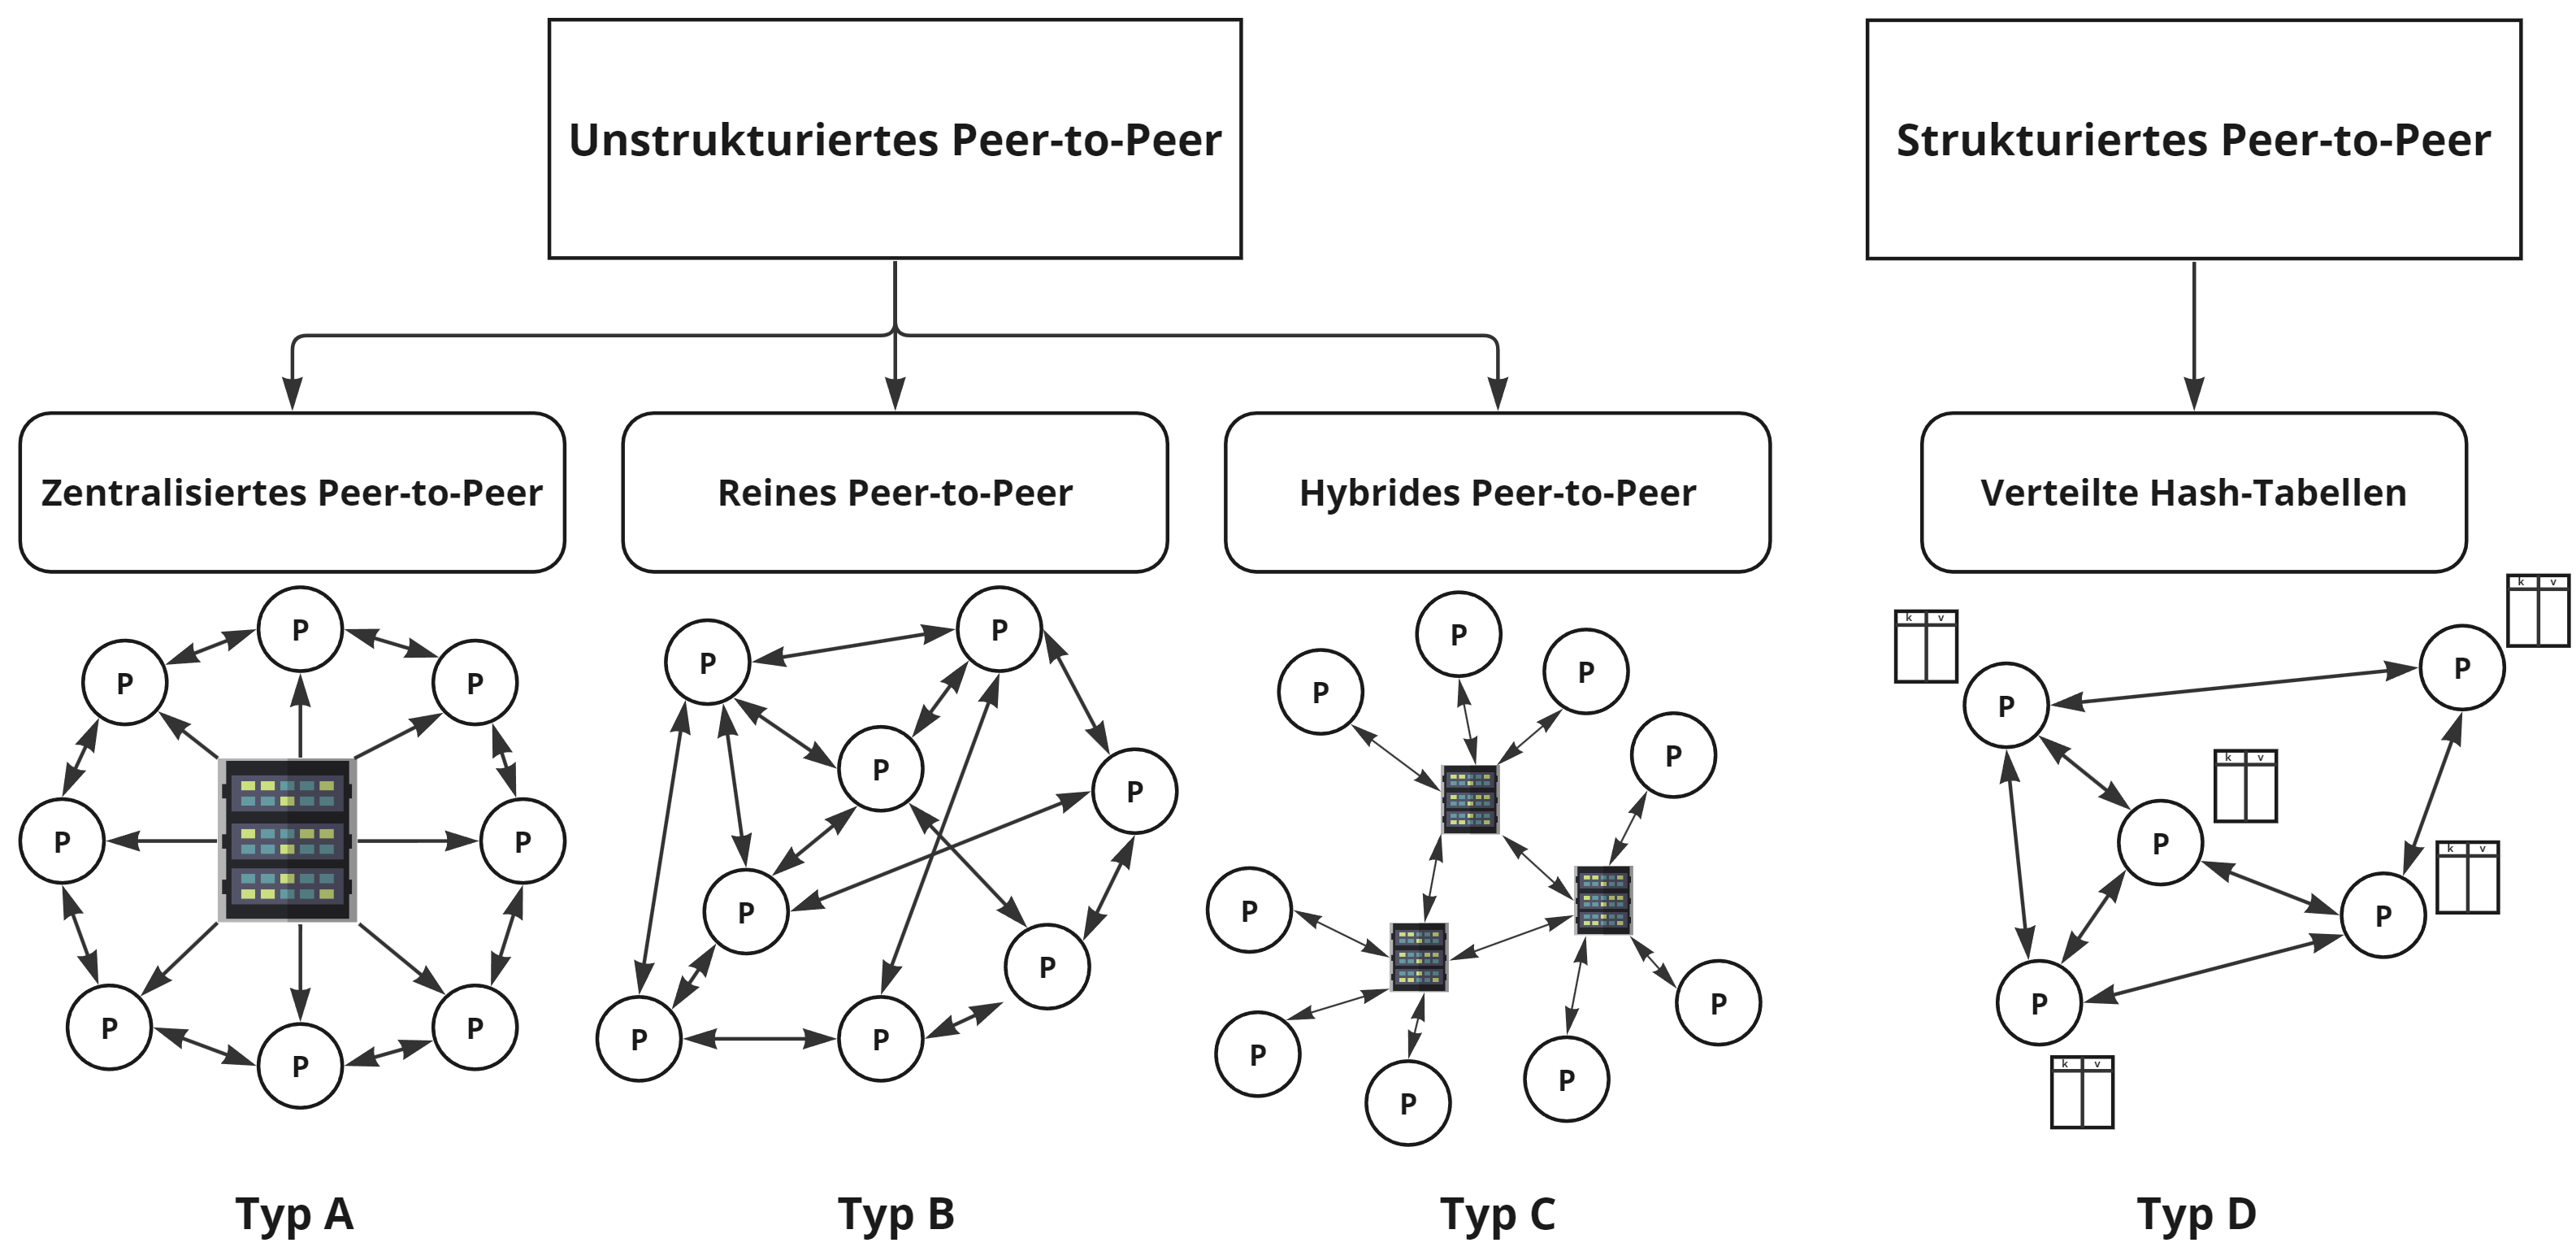
\includegraphics[width=1\linewidth]{images/p2p_typen.png}
    \captionof{figure}{Typen von Peer-to-Peer-Netzwerken, in Anlehnung an \cite[S. 363]{Luntovskyy_ModRechnernetze}}
    \label{p2p_typen}
\end{center}

\noindent Unstrukturierte und strukturierte Peer-to-Peer-Netzwerke sind unterschiedliche Ansätze zur Organisation von Knoten (engl. \textit{Nodes}) und Ressourcen in dezentralen Netzwerken.

Unstrukturierte Netzwerke sind charakterisiert durch ihre fehlende explizite Organisationsstruktur, was eine einfache Konnektivität ermöglicht. \textit{Typ A} in Abbildung \ref{p2p_typen} zeigt ein zentralisiertes Netzwerk, was bedeutet, dass alle Teilnehmer mit einem zentralen Server verbunden sind. Als Beispiel für diese Form des Peer-to-Peer dient \textit{Napster}. Bei \textit{Napster} gab es mehrere Server, die die Dateien der Teilnehmer indizierten. Die Teilnehmer konnten Dateien von anderen Teilnehmern herunterladen, indem sie eine Anfrage an einen der Server stellten, der dann die IP-Adresse des Teilnehmers zurückgab, der die Datei zur Verfügung stellte \parencite[S. 171]{Saroiu_MeasuringAndAnalyzingNapsterAndGnutellaHosts}. Diese Form ermöglicht eine schnelle und effiziente Suche nach Ressourcen, da die Ressourcen zentral verwaltet werden, aber die Abhängigkeit von einem zentralen Server macht das Netzwerk nicht skalierbar und anfällig für Ausfälle \parencite[S. 732]{Khatibi_StructuredUnstructuredP2P}.
Bei \textit{Typ B} handelt es sich um ein reines Peer-to-Peer-Netzwerk, bei dem die Teilnehmer direkt miteinander verbunden sind und jeder sowohl als Client als auch als Server fungiert \parencite[S. 732]{Khatibi_StructuredUnstructuredP2P}. Ein Beispiel für diese Form des Peer-to-Peer ist \textit{Gnutella}. Bei \textit{Gnutella} gab es keine zentrale Instanz, die die Ressourcen der Teilnehmer indizierte. Die Suche nach Ressourcen oder Informationen erfolgt durch Broadcasts oder zufällige Weiterleitungen, was jedoch zu ineffizienten Suchprozessen führen kann, da keine klare Routing-Struktur vorhanden ist \parencite[S. 171]{Saroiu_MeasuringAndAnalyzingNapsterAndGnutellaHosts}. Beim dritten und letzten Typ der unstrukturierten Netzwerke handelt es sich um ein hybrides Peer-to-Peer-Netzwerk, das Elemente aus den beiden anderen Typen kombiniert. In einem hybriden Netzwerk gibt es besondere Knoten (engl. Nodes), die die Funktionen eines Servers, wie beispielsweise Indexierung der Ressourcen, für eine bestimmte Gruppe von Teilnehmern übernehmen. Diese Knoten werden als Superknoten (engl. Super Nodes) bezeichnet. Die Super Nodes selbst sind untereinander dezentralisiert miteinander verbunden. Ein Beispiel für diese Form des Peer-to-Peer ist \textit{Gnutella2} \parencite[S. 732]{Khatibi_StructuredUnstructuredP2P}. 

Strukturierte Peer-to-Peer-Netzwerke hingegen weisen klare Regeln und Algorithmen zur Organisation der Knoten auf. Diese Netzwerke verfügen über eine explizite Organisationsstruktur, sei es eine Ringstruktur, k-bucket basierte Systeme oder andere, die es ermöglichen, effizientes Routing und eine optimierte Ressourcenverwaltung zu erreichen. Durch diese klar definierte Struktur sind strukturierte Netzwerke oft stabiler und bieten eine effizientere Ressourcenlokalisierung im Vergleich zu ihren unstrukturierten Gegenstücken. Allerdings kann diese Stabilität auf Kosten von Flexibilität und Anpassungsfähigkeit gehen, da Änderungen in der Netzwerktopologie oder hohe Dynamik der Knoten schwerer zu handhaben sind \parencite[S. 40]{Vu_P2PComputing}.


\subsection{Problemstellung und mögliche Lösungen}

Peer-to-Peer-Netzwerke sind nicht ohne Probleme. Die dezentrale Struktur der Netzwerke bringt einige Herausforderungen mit sich, die es zu bewältigen gilt. Eines der Probleme stellen die \textit{Network Address Translators} (kurz: NATs) dar. NATs sind dafür zuständig, private IP-Adressen in öffentliche IP-Adressen umzuwandeln und umgekehrt. Sie werden in Routern oder Gateways eingesetzt und dienen dazu, den Zugang von Geräten im lokalen Netzwerk (die private IP-Adressen verwenden) zum Internet zu ermöglichen, indem sie den Datenverkehr zwischen dem lokalen Netzwerk und dem externen Netzwerk, wie dem Internet, verwalten. Peer-to-Peer Verbindungen stoßen bei Network Address Translators oft auf Probleme, was daran liegt, dass NATs normalerweise nicht erlauben, dass externe Geräte direkt mit internen kommunizieren. Zudem werden Ports dynamisch für ausgehenden Traffic zugewiesen, was das Weiterleiten eingehender Verbindungen erschwert. Symmetrische NATs verschärfen dieses Problem, da sie für ausgehende Verbindungen eine eindeutige Kombination von IP-Adresse und Port verwenden, die sich bei jeder neuen Verbindung ändert \Parencite[S. 1-9]{rfc2663_NAT_Terminology}.

Dies ist ein Problem, da die Teilnehmer nicht direkt miteinander kommunizieren können, wenn sie sich hinter einem NAT befinden. Um dieses Problem zu lösen, gibt es verschiedene Lösungsansätze. Einer davon ist das \textit{Relaying}. Beim Relaying wird ein Server als Vermittler zwischen den Teilnehmern verwendet. Die Teilnehmer verbinden sich mit dem Server und leiten ihren Datenverkehr über diesen Server weiter. 
Ein weiterer Ansatz ist die \textit{Connection Reversal}. Bei der Connection Reversal wird ein \textit{Rendezvous-Server} verwendet, um eine Verbindung zwischen den Teilnehmern herzustellen. Der Teilnehmer hinter dem NAT verbindet sich mit dem Rendezvous-Server und teilt diesem seine öffentliche IP-Adresse und Port mit. Der andere Teilnehmer verbindet sich ebenfalls mit dem Rendezvous-Server und erhält die IP-Adresse und Port des  Teilnehmers hinter dem NAT. Bei dieser Technik darf sich nur einer der Teilnehmer hinter einem NAT befinden.
\textit{Hole Punching} beschreibt einen weiteren Lösungsansatz. Zwei Geräte, die eine direkte Verbindung miteinander aufbauen möchten, initiieren gleichzeitig eine Verbindung zu einem Server, der sich außerhalb des NATs befindet. Der Server sammelt die IP-Adressen und Ports der beiden Geräte und leitet diese an die jeweils andere Partei weiter. Die beiden Geräte versuchen dann, eine Verbindung zueinander herzustellen, indem sie gleichzeitig Datenpakete an die IP-Adresse und den Port des anderen Geräts senden. Dabei wird versucht, das NAT dazu zu bringen, die Verbindung zu öffnen, indem es die ankommenden Pakete als Antwort auf die ausgehenden Pakete erkennt. Wenn dies gelingt, wird ein temporäres Loch im NAT geöffnet, das es den Geräten ermöglicht, direkt miteinander zu kommunizieren. Diese Technik erfordert eine präzise Koordination und die Fähigkeit der beiden Geräte zur gleichen Zeit Datenpakete zu senden und zu empfangen. Zudem ist es nicht immer möglich, ein temporäres Loch im NAT zu öffnen, da es von der Implementierung des NATs abhängt. Eine Abwandlung vom Hole Punching ist die \textit{Port Number Prediction}. Hierbei wird versucht, die Portnummer vorherzusagen, die das NAT für die Verbindung verwenden wird.Durch Beobachtung und Analyse vorheriger Verbindungen wird versucht Muster oder Trends in der Art und Weise zu erkennen, wie Portnummern zugewiesen werden. Dies könnte auf bestimmte Algorithmen oder Verhaltensweisen des Systems hinweisen, woraus dann die Portnummer vorhergesagt werden kann. Diese Technik ist jedoch nicht immer zuverlässig, da es rein auf Annahmen basiert und das Risiko besteht, dass sich das Portzuweisungsmuster jederzeit ändert \Parencite[S. 7-21]{rfc5128_P2P_NATs}.


Um die Problematik von Peer-to-Peer-Netzwerken zu lösen, können verschiedene Protokolle zum Einsatz kommen. Eines dieser Protokolle ist STUN (Session Traversal Utilities for NAT). STUN ist ein Netzwerkprotokoll, das es Geräten, die sich hinter einem NAT befinden, ermöglicht, ihre öffentliche IP-Adresse und Port zu ermitteln. Es bietet an sich keine Möglichkeit für eine Umgehung des NATs, sondern ist dafür gedacht, als eines von mehreren Werkzeugen verwendet zu werden, um ein NAT zu umgehen. Mittels STUN lässt sich nur ermitteln, ob sich ein Gerät hinter einem NAT befindet und welche IP-Adresse und Port es verwendet \parencite[S. 4]{rfc8489_STUN}.

TURN (Traversal Using Relays around NAT) ist ein weiteres Netzwerkprotokoll, das im Zusammenhang mit NATs verwendet wird. Aus der Spezifikation ist zu entnehmen, dass TURN ein Protokoll ist, das es Geräten, die sich hinter einem NAT befinden, ermöglicht, eine Verbindung zu einem anderen Gerät herzustellen, indem es einen Server als Vermittler verwendet. TURN ist ein Protokoll, das auf STUN aufbaut. Es bietet die gleichen Funktionalitäten wie STUN, aber zusätzlich die Möglichkeit, den Datenverkehr über einen Server zu leiten, um eine Verbindung zwischen zwei Geräten herzustellen. Das funktioniert auch, wenn sich beide Geräte hinter einem NAT befinden \parencite[S. 7]{rfc8656_TURN}.

ICE (Interactive Connectivity Establishment) ist ein Framework, das mehrere Techniken kombiniert, um eine Verbindung zwischen zwei Endpunkten herzustellen, die sich hinter NATs befinden. Es verwendet STUN und TURN, um die öffentliche IP-Adresse und Port eines Geräts zu ermitteln und den Datenverkehr über einen Server zu leiten \Parencite[S. 6]{rfc8445_ICE}.


\subsection{Overlay-Netzwerke}

Peer-to-Peer-Netzwerke können als Overlay-Netzwerke betrachtet werden. Ein Overlay-Netzwerk ist ein virtuelles Netzwerk, das, wie in Abbildung \ref{overlay_network} (\textit{\nameref{overlay_network}}) zu sehen ist, über ein physisches Netzwerk gelegt wird.

\begin{center}
    \captionsetup{type=figure}
    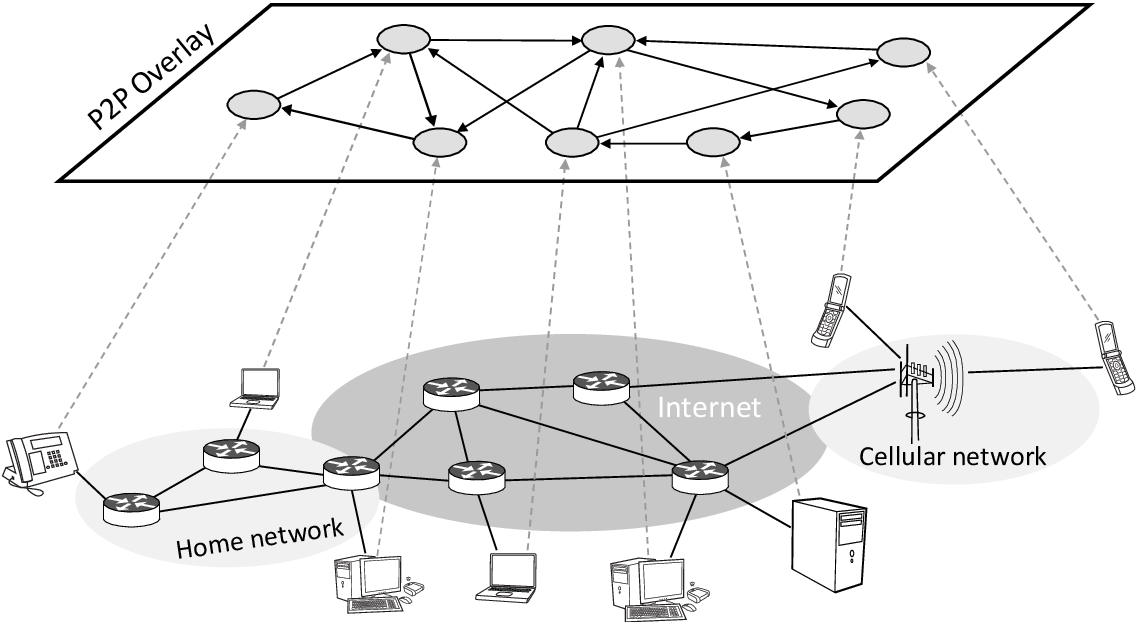
\includegraphics[width=0.9\linewidth]{images/overlay_network.png}
    \captionof{figure}{Peer-to-Peer-Overlay-Netzwerk mit darunterliegendem physischen Netzwerk \parencite{Kunzmann_OverlayNetworksImageSource}}
    \label{overlay_network}
\end{center}

\noindent In diesem Fall ist das physische Netzwerk das Internet. Das Overlay-Netzwerk ist eine logische Struktur, die es ermöglicht, die Kommunikation zwischen den Teilnehmern zu organisieren. Es besteht aus einer Reihe von Knoten, die über eine logische Verbindung miteinander verbunden sind. Die Verbindungen zwischen den Knoten werden durch Routing-Algorithmen verwaltet \parencite{Lua_P2POverlayNetworksPaper}.

Beispiele für Routing-Algorithmen sind \textit{Kademlia}, \textit{Chord} und \textit{Pastry}. Diese drei Algorithmen verwenden sogenannte \textit{Distributed Hash Tables}, um die Knoten zu verwalten. \textit{Distributed Hash Tables} (kurz: DHTs) sind verteilte Datenstrukturen, die in Peer-to-Peer-Netzwerken verwendet werden, um effizient Schlüssel-Wert-Paare zu speichern und abzurufen. Anders als herkömmliche zentralisierte Datenbanken oder Speicherlösungen benötigen DHTs keinen zentralen Server zur Speicherung oder Verwaltung von Daten. Sie funktionieren auf Basis von Hash-Funktionen, die einen Schlüssel in einen eindeutigen Hash umwandeln. Diese Hashes dienen als Adressen, um zu bestimmen, wo die entsprechenden Daten im Netzwerk gespeichert sind. Die Daten werden über verschiedene Peers im Netzwerk verteilt, wobei jeder Peer nur einen Teil der Daten basierend auf seinem Verantwortungsbereich speichert . Um effizient auf die gespeicherten Daten zuzugreifen, verwenden DHTs  Routing-Algorithmen wie Pastry, Kademlia oder Chord. Diese Algorithmen ermöglichen es, Peers im Netzwerk zu finden, die für die Speicherung oder Abfrage von Daten zuständig sind, selbst wenn sich die Netzwerktopologie ständig verändert. Ein großer Vorteil von DHTs ist ihre Skalierbarkeit. Sie können mit der Netzwerkgröße wachsen, ohne an Effizienz zu verlieren. Neue Peers können nahtlos hinzugefügt werden, und die Struktur der DHT passt sich dynamisch an Veränderungen im Netzwerk an \parencite[S. 43-46]{Balakrishnan_LookingUpDataInP2PSystems} \parencite[postnote]{Stoica_Chord,Rowstron_Pastry,Maymounkov_Kademlia}.


\subsection{Kademlia vs. Chord vs. Pastry}

\textit{Kademlia} ist ein Peer-to-Peer-Protokoll, das für die Organisation von Knoten in einem Netzwerk verwendet wird. Es ist ein strukturiertes Peer-to-Peer-Netzwerk, das auf einer K-Bucket-Struktur basiert. Die K-Buckets enthalten eine Liste von Knoten für verschiedene Schlüsselbereiche basierend auf ihrer Nähe, die durch XOR-Distanzen der IDs berechnet wird. Die Verbindungen zwischen den Knoten sind asymmetrisch, und jeder Knoten speichert Informationen über andere Knoten in seinen K-Buckets. Bei der Suche nach einem bestimmten Schlüssel erfolgt das Routing durch die XOR-Entfernung, wodurch die nächsten Knoten für diesen Schlüssel gefunden werden. Dieses Verfahren ermöglicht eine logarithmische Anzahl von Schritten für die Suche und bietet eine robuste Struktur, die gut mit dynamischen Netzwerkänderungen umgehen kann \parencite[S. 1-2]{Maymounkov_Kademlia}.

\textit{Chord} ist ein weiteres Peer-to-Peer-Protokoll, das für die Organisation von Knoten in einem Netzwerk verwendet wird. Es ist ebenfalls ein strukturiertes Peer-to-Peer-Netzwerk, basiert allerdings auf einer Ringstruktur. Die Knoten sind in einem Ring angeordnet und jeder Knoten ist für einen bestimmten Schlüsselbereich verantwortlich. Die Verbindungen zwischen den Knoten sind durch ihren Platz im Ring definiert, wobei jeder Knoten eine Verbindung zu seinem nächsten Nachbarn im Uhrzeigersinn hat. Bei der Suche nach einem bestimmten Schlüssel durchläuft eine Anfrage einen logarithmischen Pfad im Ring, wobei die Knoten auf dem Weg begrenzte Informationen über andere Knoten behalten, um Anfragen weiterzuleiten. Dieses Modell ist recht einfach und effizient für viele Anwendungsfälle, aber es könnte anfällig sein für Engpässe oder längere Suchzeiten, insbesondere wenn das Netzwerk dynamisch ist und sich die Konfiguration häufig ändert \parencite[S. 1-2]{Stoica_Chord}.

Auch \textit{Pastry} basiert auf einer Ringstruktur und ist darauf ausgerichtet, die Übertragung von Daten und die Suche nach Peers in großen, dynamischen Netzwerken zu optimieren. Im Kern funktioniert Pastry wie folgt: Es organisiert Peers in einem virtuellen Ring, wobei jeder Peer eine eindeutige ID hat. Diese IDs sind im metrischen Raum angeordnet, wodurch ähnliche IDs oder Schlüssel ähnliche Peers im Ring finden. Jeder Peer in Pastry verfügt über Routing-Tabellen, die Informationen über andere Peers im Ring enthalten, die in der Nähe ihrer eigenen ID liegen. Diese Routing-Tabellen ermöglichen es, Peers in logarithmischer Zeit zu erreichen, unabhängig von der Netzwerkgröße. Wenn eine Nachricht gesendet werden soll, wählt der Sender anhand der Ziel-ID des Peers den nächsten Peer in seiner Routing-Tabelle aus, der der Ziel-ID am nächsten liegt. Diese Prozedur wird iterativ wiederholt, bis die Nachricht ihren Ziel-Peer erreicht hat. Pastry ist widerstandsfähig gegen Ausfälle und kann sich an dynamische Netzwerkänderungen anpassen, indem es die Routing-Struktur und -Tabellen entsprechend aktualisiert \parencite[S. 331-339]{Rowstron_Pastry}.


Für den Anwendungsfall des Instant Messaging ist die effektive Bewältigung von \textit{Churn} von entscheidender Bedeutung. Churn bezieht sich auf die häufigen Ein- und Austritte von Teilnehmern in einem Peer-to-Peer-Netzwerk. In einem Instant Messaging Kontext bedeutet dies, dass Benutzer sich ständig anmelden oder abmelden. Ein Protokoll, das gut mit Churn umgehen kann, ist entscheidend, um eine zuverlässige und nahtlose Kommunikation zu gewährleisten. Das richtige Handling von Churn ist daher ein Schlüsselfaktor für die Leistungsfähigkeit und Stabilität eines Instant Messaging Protokolls \parencite[S. 316-317]{Peris_KademliaChurn}.

Kademlia ist bekannt für seine Effizienz bei der Skalierung und der Robustheit gegenüber Churn. Es verwendet eine XOR-Metrik, um Peers in einem logarithmischen Adressraum zu organisieren, was zu kurzen Pfaden für Anfragen führt. Dadurch eignet es sich gut für große, dynamische Netzwerke, da es leicht neue Peers integrieren und Ausfälle tolerieren kann \Parencite{MedranoChavez_ChordKademliaHighChurnScenarios}.

Chord hingegen basiert, wie bereits angesprochen, auf einem ringförmigen Adressraum, in dem jeder Peer für eine bestimmte Adresse verantwortlich ist. Es bietet eine deterministische Routing-Tabelle und erfordert im Vergleich zu Kademlia weniger Overhead für Routinginformationen. Dies macht Chord gut geeignet für statischere Netzwerke, in denen die Stabilität der Routinginformationen wichtiger ist als die Anpassungsfähigkeit an dynamische Veränderungen \parencite{Stoica_Chord}.

Pastry verwendet eine gemeinsame Präfix-Länge als Grundlage für die Adressierung und organisiert Peers in einem eindimensionalen Raum. Es bietet eine gute Balance zwischen Effizienz und Skalierbarkeit, indem es kurze Routingpfade mit geringem Overhead ermöglicht. Pastry eignet sich gut für mittelgroße Netzwerke mit moderater Dynamik und bietet eine solide Leistung bei der Bewältigung von Knotenausfällen \parencite{Rowstron_Pastry}.

Insgesamt bieten alle drei Algorithmen Lösungen für verteilte Systeme, variierend in ihrer Anpassungsfähigkeit, Skalierbarkeit und Effizienz je nach den spezifischen Anforderungen des Netzwerks. Die Wahl zwischen Kademlia, Chord und Pastry hängt von Faktoren wie der Größe des Netzwerks, der erwarteten Dynamik (Churn) und der Priorität zwischen Skalierbarkeit und Routingstabilität ab.

\subsection{Angriffe auf Peer-to-Peer-Netzwerke}

\subsubsection{Denial-of-Service-Angriff}

Mit einem \textit{Denial-of-Service}-Angriff (kurz: \textit{DoS-Angriff}) wird versucht, die Verfügbarkeit eines Dienstes zu beeinträchtigen, indem die Ressourcen des Dienstes erschöpft werden, sodass diese ausfallen \parencite{Bicakci_DoSAttacks}. In einem Peer-to-Peer-Netzwerk kann ein DoS-Angriff auf verschiedene Arten durchgeführt werden. Eine Möglichkeit ist es, einen Peer mit Anfragen zu überfluten, um ihn zu überlasten. Eine andere Möglichkeit ist es, einen Peer mit gefälschten Informationen zu überfluten, um ihn zu täuschen. Beide Methoden führen dazu, dass der Peer nicht mehr in der Lage ist, seine Aufgaben zu erfüllen, was zu einem Ausfall des Dienstes führt. Dieser Angriff wird noch effektiver, wenn er von mehreren Angreifern gleichzeitig durchgeführt wird. Dies wird als \textit{Distributed Denial-of-Service}-Angriff (kurz: \textit{DDoS-Angriff}) bezeichnet. Bei einem DDoS-Angriff wird der Peer mit Anfragen von mehreren Angreifern überflutet, was es schwieriger macht, den Angriff zu stoppen \Parencite[S. 6]{Baptiste_AttacksOnP2PNetworks}.


\subsubsection{Sybil-Angriff}
\label{subsubsec:sybil_attack_p2p}

Der Sybil-Angriff ist nicht spezifisch für Blockchain, sondern kann in jedem Peer-to-Peer-Netzwerk durchgeführt werden. Bei diesem Angriff erstellt ein einzelner Angreifer mehrere Identitäten, um die Kontrolle über das Netzwerk zu erlangen. Der Angreifer kann dann die Kontrolle über das Netzwerk übernehmen, indem er die Mehrheit der Identitäten kontrolliert \parencite[S. 251]{Douceur_SybilAttack}. Nach einer erfolgreichen Übernahme von Teilen des Netzwerks, besteht die Möglichkeit der Durchführung eines \textit{Eclipse}-Angriffs, welcher im nächsten Abschnitt erklärt wird \parencite[S. 13-15]{Baptiste_AttacksOnP2PNetworks}.


\subsubsection{Eclipse-Angriff}
\label{subsubsec:eclipse_attack_p2p}

Bei einem \textit{Eclipse}-Angriff wird versucht, einen Peer von allen anderen Peers im Netzwerk zu isolieren. Dies wird erreicht, indem bereits durch den vorhergegangenen Sybil-Angriff die Mehrheit der Peers kontrolliert wird. Der Angreifer kann dann die Verbindungen des Opfers zu anderen Peers im Netzwerk verhindern, indem er die Verbindungen zu anderen Peers kontrolliert \Parencite[S. 14]{Baptiste_AttacksOnP2PNetworks}. 



\section{Sicherheit}
\label{sec:sicherheit_basics}

Wie aus der Abbildung in Abschnitt \ref{subsec:overlay_netzwerke} \textit{\nameref{subsec:overlay_netzwerke}} ersichtlich ist, ist das Overlay-Netzwerk die oberste Schicht des Peer-to-Peer-Netzwerks. Es sorgt dafür, dass sich die Teilnehmer des Netzwerks finden können. Die eigentliche Kommunikation, also das Senden und Empfangen von Nachrichten, erfolgt jedoch über das Internet. Da das Internet ein öffentliches Netzwerk ist, besteht die Gefahr, dass die Nachrichten abgefangen und mitgelesen werden können. Die Nachrichten müssen über Verteilerknoten oder Access Points übertragen werden, die nicht vertrauenswürdig sind. Um ein Mitlesen oder Verändern der Nachrichten zu verhindern, muss die Kommunikation abgesichert werden. 

Mittels Kryptografie kann die Vertraulichkeit, Integrität und Authentizität der Kommunikation gewährleistet werden \Parencite[S. 7]{Hellmann_IT-Sicherheit}.


\subsection{Vertraulichkeit}
\label{subsec:vertraulichkeit_basics}

Die Vertraulichkeit der Kommunikation wird durch Verschlüsselung gewährleistet. Man unterschiedet zwei Formen der Kryptografie: \textit{symmetrische} und \textit{asymmetrische} Kryptografie. Bei der \textit{symmetrischen} Kryptografie wird ein und derselbe Schlüssel zum Verschlüsseln und Entschlüsseln der Nachricht verwendet. Der Sender der Nachricht verschlüsselt die Nachricht mit einem Schlüssel und sendet die nun verschlüsselte Nachricht an den Empfänger. Der Empfänger kann die Nachricht mit dem gleichen Schlüssel entschlüsseln. Dadurch kann ein Angreifer, der die Nachricht abfängt, diese nicht entschlüsseln, da er den Schlüssel nicht kennt. Abbildung \ref{fig:symmetrische_verschluesselung} zeigt den Ablauf der symmetrischen Verschlüsselung.

\begin{center}
    \captionsetup{type=figure}
    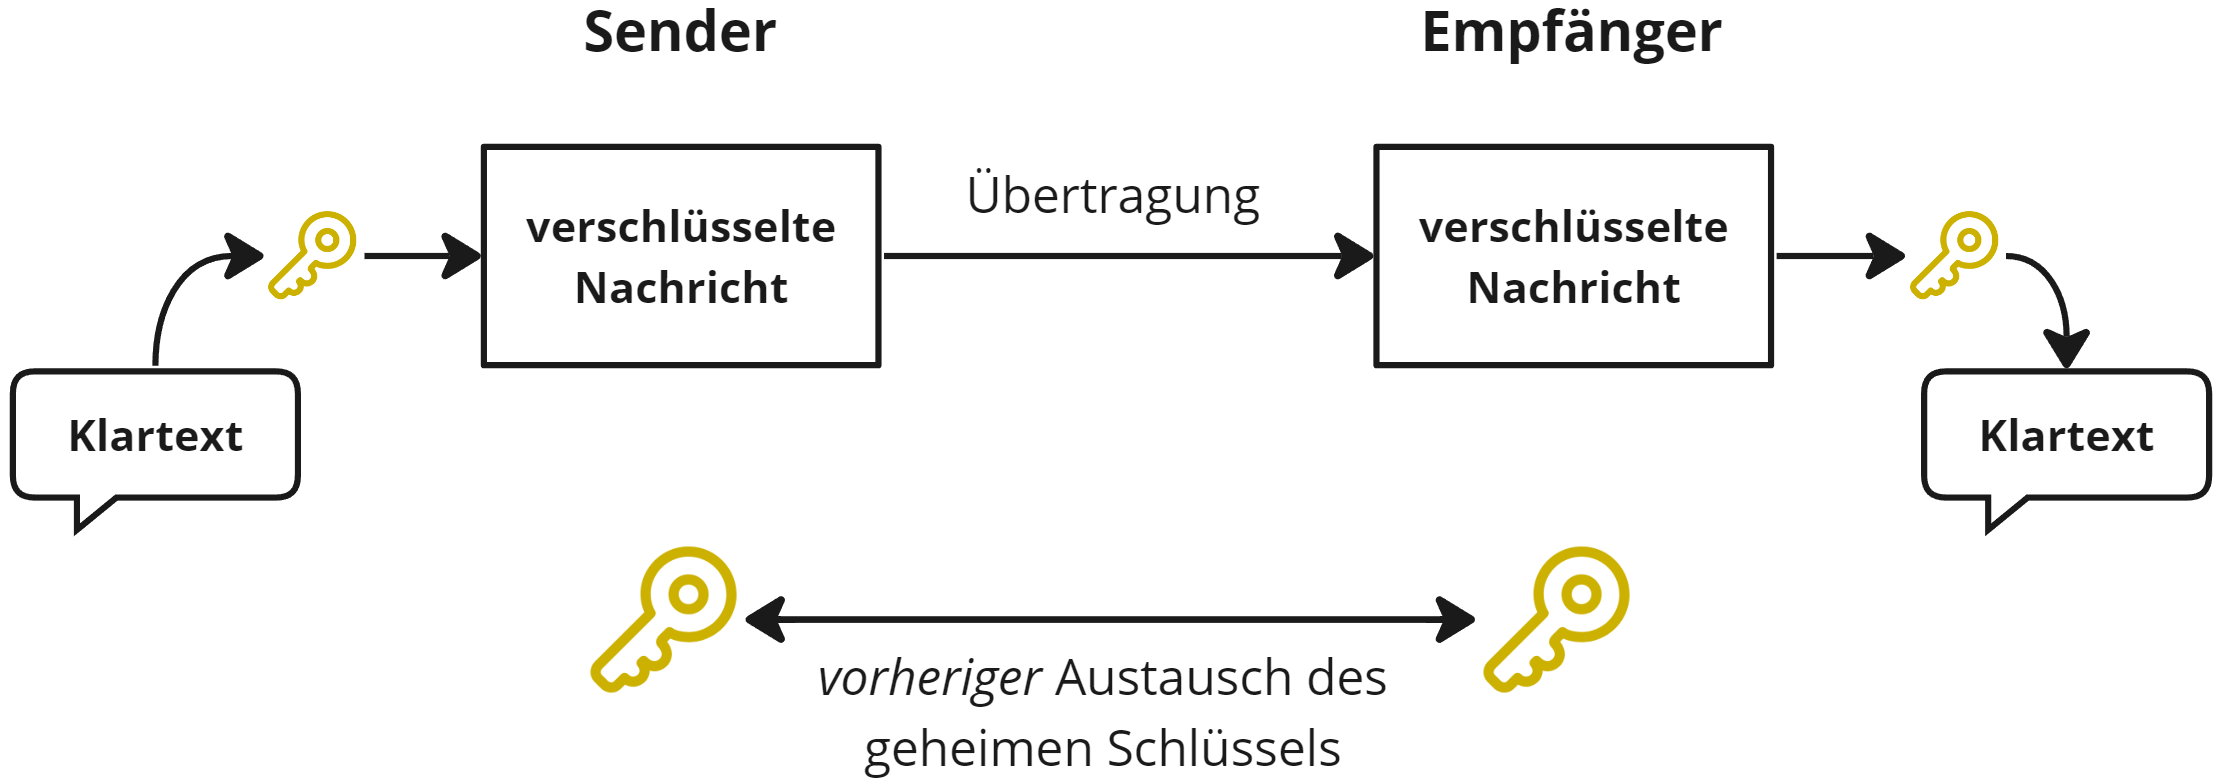
\includegraphics[width=1\linewidth]{images/symmetric_encryption.png}
    \caption{Symmetrische Verschlüsselung (in Anlehnung an \cite{ElektronikKompendium_symmetrischeVerschluesselung})}
    \label{fig:symmetrische_verschluesselung}
\end{center}

\noindent Das Problem bei der symmetrischen Kryptografie ist, dass der Schlüssel zu Beginn der Kommunikation vom Sender an den Empfänger gelangen muss. Dies stellt eine Herausforderung dar, wenn Sender und Empfänger sich noch nicht kennen und noch nie zuvor miteinander kommuniziert haben oder noch nicht über andere Wege einen Schlüssel ausgetauscht haben. Sollte der Schlüssel bei der Übertragung über einen unsicheren Kanal abgefangen werden, kann der Angreifer die Kommunikation entschlüsseln und somit mitlesen \Parencites[S. 644]{DiffieHellman_NewDirectionsInCryptography}[S. 5-8]{Wong_KryptoPraxis}. 

In diesem Fall kann eine Schlüsselvereinbarung verwendet werden, um einen gemeinsamen Schlüssel zu erhalten. Bei der Schlüsselvereinbarung wird ein Schlüssel zwischen zwei Parteien vereinbart, ohne dass dieser über einen unsicheren Kanal übertragen werden muss \Parencite[S. 102]{Wong_KryptoPraxis}. Abbildung \ref{fig:schluesselvereinbarung} zeigt den Ablauf der Schlüsselvereinbarung.

\begin{center}
    \captionsetup{type=figure}
    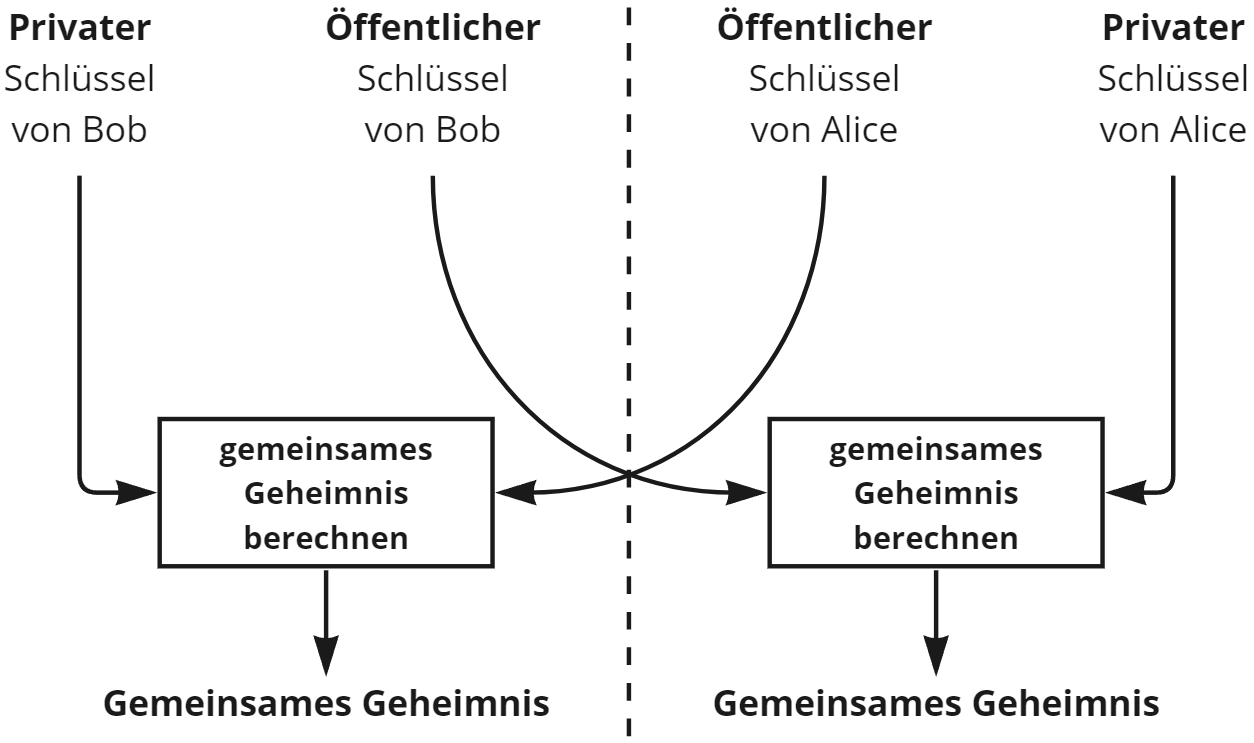
\includegraphics[width=0.7\linewidth]{images/key_exchange.png}
    \caption{Schlüsselvereinbarung (in Anlehnung an \cite[S. 102]{Wong_KryptoPraxis})}
    \label{fig:schluesselvereinbarung}
\end{center}

\noindent Beide Teilnehmer generieren einen privaten Schlüssel und einen öffentlichen Schlüssel. Durch die Kombination des öffentlichen Schlüssels des anderen Teilnehmers und des eigenen privaten Schlüssels wird ein gemeinsames Geheimnis berechnet. Dieses gemeinsame Geheimnis kann dann für die symmetrische Verschlüsselung verwendet werden, da dadurch beide Teilnehmer den gleichen Schlüssel besitzen \Parencite[S. 102]{Wong_KryptoPraxis}.


Bei der \textit{asymmetrische} Kryptografie (auch \textit{Public-Key-Kryptografie} genannt) wird anstatt nur eines Schlüssels ein Schlüsselpaar generiert, das aus einem öffentlichen und einem privaten Schlüssel besteht. Der öffentliche Schlüssel des Empfängers wird zum Verschlüsseln der Nachrichten verwendet und zum Entschlüsseln der Nachrichten wird der private Schlüssel des Empfängers verwendet. Der öffentliche Schlüssel des Empfängers kann von jedem verwendet werden, um Nachrichten an den Empfänger zu verschlüsseln. Nur der Empfänger kann die Nachrichten entschlüsseln, da nur er den privaten Schlüssel besitzt. Der Ablauf der asymmetrischen Verschlüsselung ist in Abbildung \ref{fig:asymmetrische_verschluesselung} dargestellt.


\begin{center}
    \captionsetup{type=figure}
    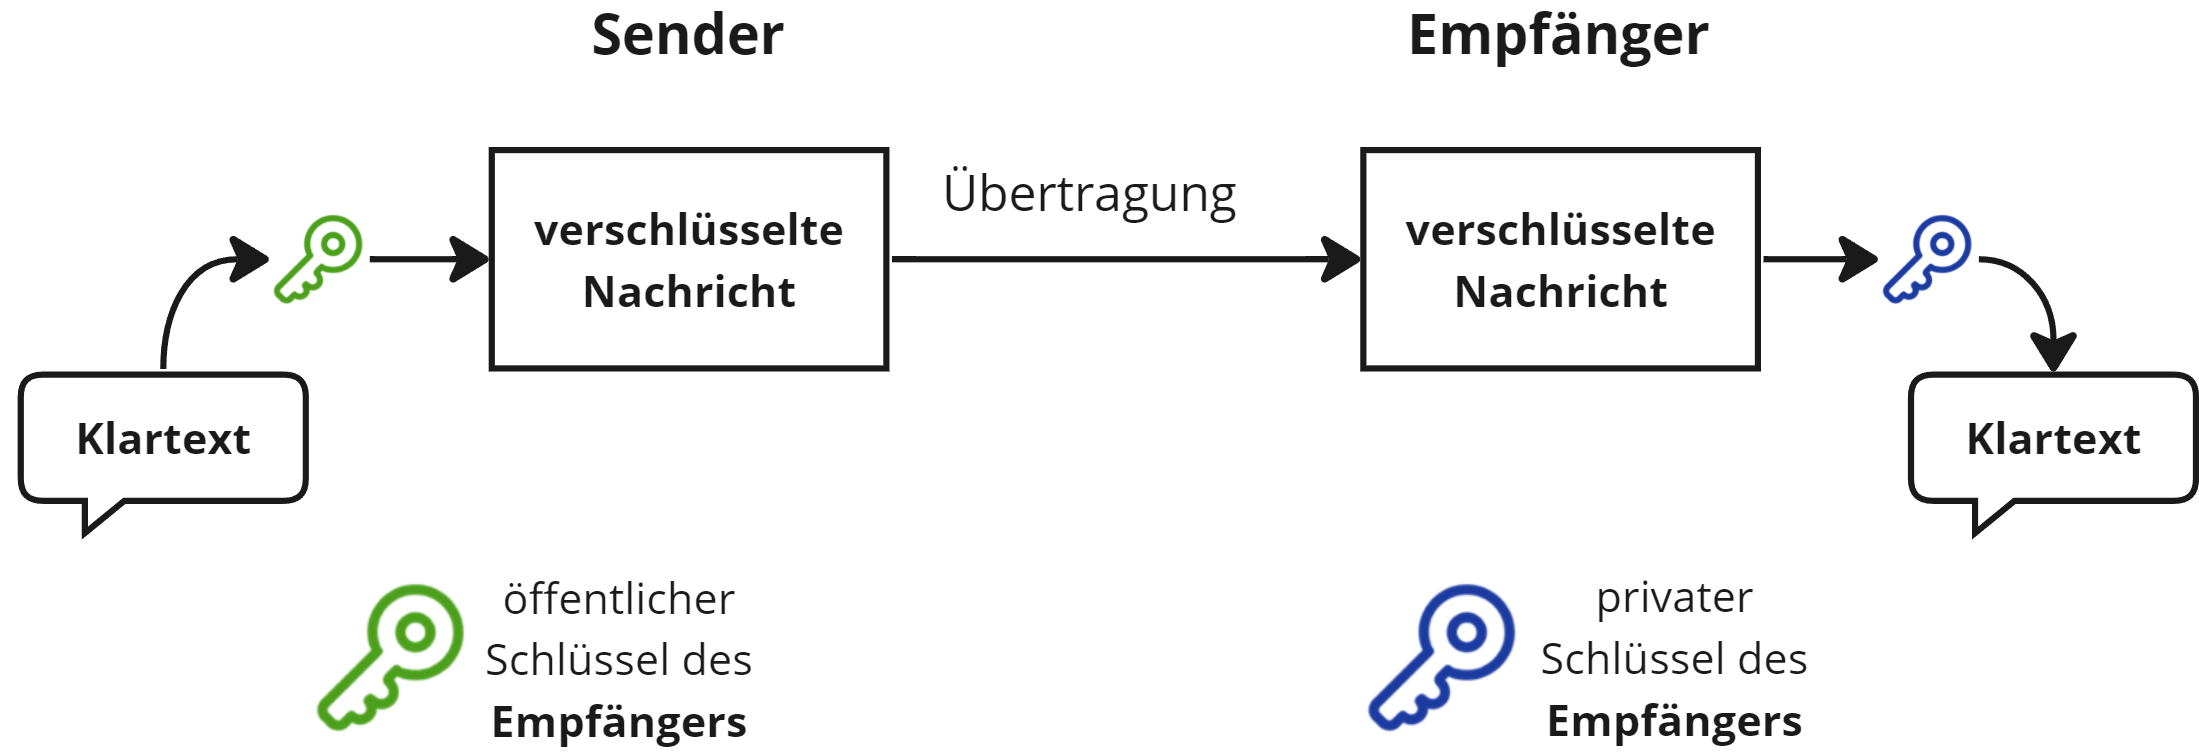
\includegraphics[width=1\linewidth]{images/asymmetric_encryption.png}
    \caption{Asymmetrische Verschlüsselung (in Anlehnung an \cite{ElektronikKompendium_asymmetrischeVerschluesselung})}
    \label{fig:asymmetrische_verschluesselung}
\end{center}

\noindent Es ist außerdem nicht möglich, Nachrichten, die mit dem öffentlichen Schlüssel verschlüsselt wurden, mit diesem auch wieder zu entschlüsseln \parencite{ElektronikKompendium_asymmetrischeVerschluesselung}. 

Diese kryptografische Verfahren können kombiniert werden, um die Vorteile von diesen zu nutzen. Der Schlüsselaustausch wird mit der asymmetrischen Verschlüsselung durchgeführt und die eigentliche Kommunikation wird mit der symmetrischen Verschlüsselung durchgeführt.


\subsection{Integrität}
\label{subsec:integritaet_signatur}

Um die Integrität der Kommunikation zu gewährleisten, wird Hashing verwendet. Das Hashing von Daten erfordert die Verwendung einer \textit{Hash-Funktion}. Hash-Funktionen sind Funktionen, die eine Eingabe beliebiger Länge in eine Ausgabe fester Länge umwandeln. Dabei ist es wichtig, dass die Hash-Funktion zwei Eigenschaften erfüllt: \textit{Einwegfunktion} und \textit{Kollisionsresistenz}. Eine Hash-Funktion erfüllt die Eigenschaft der Einwegfunktion, wenn es nicht möglich ist, von der Ausgabe auf die Eingabe zu schließen. Das bedeutet, dass es nicht möglich ist, aus dem Hash-Wert die ursprünglichen Daten zu rekonstruieren. Die Eigenschaft der Kollisionsresistenz ist erfüllt, wenn es nicht möglich ist, zwei verschiedene Eingaben zu finden, die auf den gleichen Hash-Wert abgebildet werden \parencites[S. 12-13]{Brünnler_BlockchainKurzGut}[S. 6]{Fill_BlockchainGrundlagen}.

Das Ergebnis der Hash-Funktion ist eine Zeichenkette, die aus einer festen Anzahl an Zeichen besteht und als \textit{Hash-Wert} oder auch nur \textit{Hash} bezeichnet wird. Der Hash-Wert ist ein eindeutiger Fingerabdruck der Daten, die in die Hash-Funktion eingegeben wurden. Sollte sich also der Inhalt der Daten ändern, ändert sich auch der Hash-Wert. 


\subsection{Authentizität}

In Kombination mit einer sogenannten Signatur kann zusätzlich zur Integrität auch die Authentizität einer Nachricht gewährleistet werden. Abbildung \ref{fig:signatur} zeigt, wie eine Nachricht digital signiert wird.

\begin{center}
    \captionsetup{type=figure}
    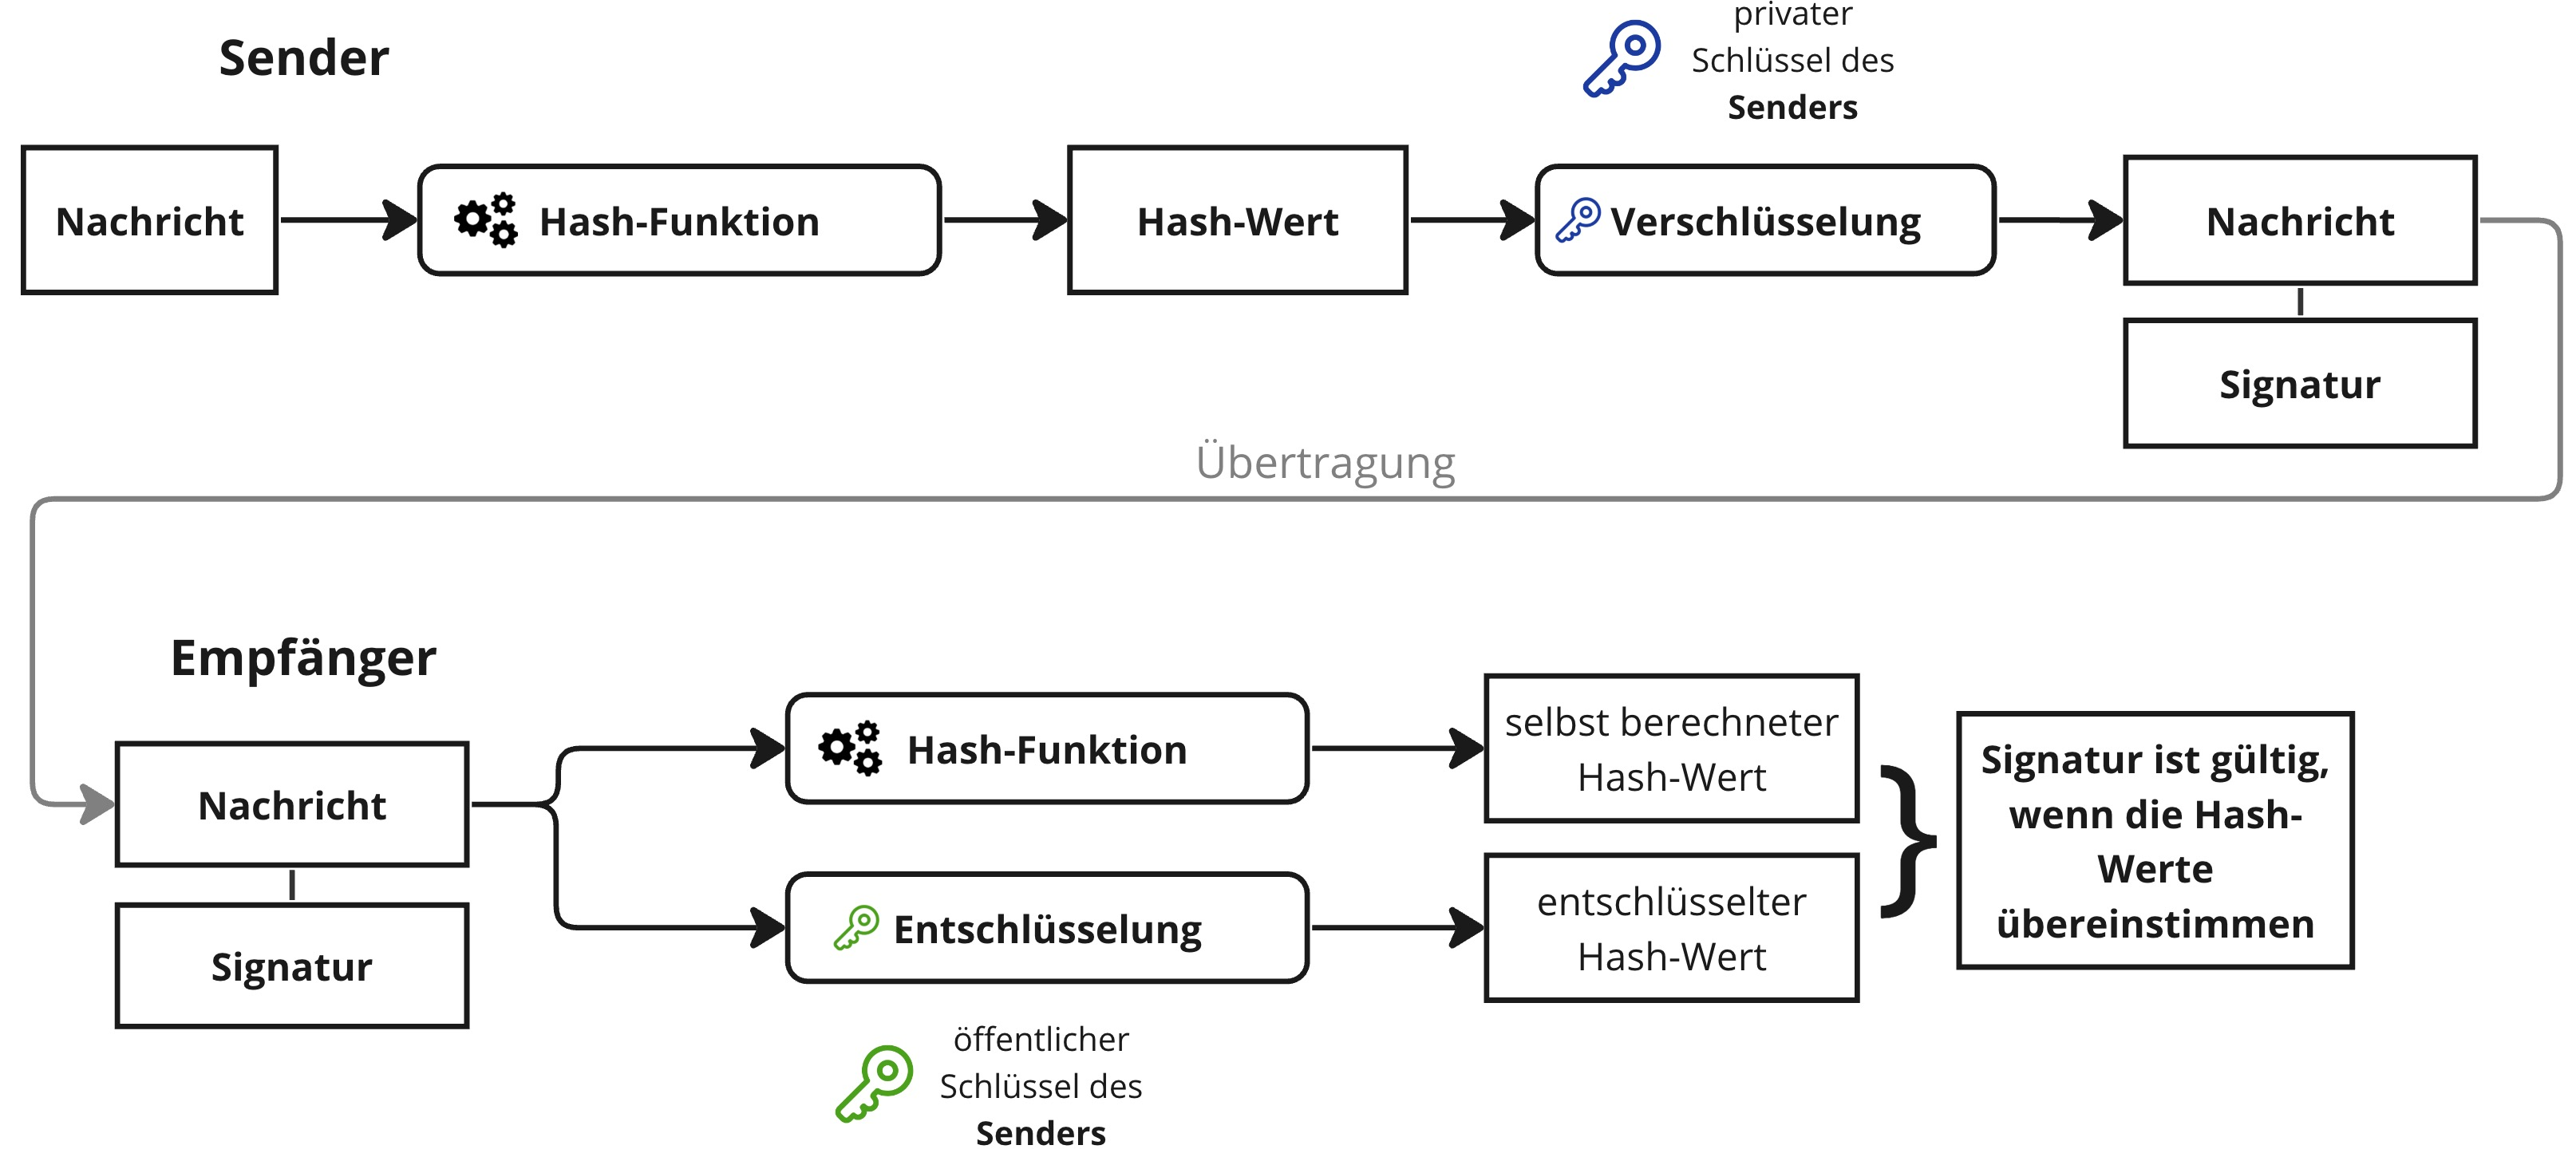
\includegraphics[width=1\linewidth]{images/signatur_2.jpg}
    \caption{Signieren einer Nachricht (in Anlehnung an \cite{DocuSign_digitaleSignaturen})}
    \label{fig:signatur}
\end{center}


\noindent Der Sender berechnet den Hash-Wert der Nachricht, verschlüsselt diesen mit seinem privaten Schlüssel. Das Ergebnis ist die digitale Signatur, welche an die Nachricht angehängt wird. Der Empfänger braucht den öffentlichen Schlüssel des Senders, um die Signatur zu entschlüsseln. Dafür gibt es verschiedene Möglichkeiten. Eine Möglichkeit ist, dass der Sender den öffentlichen Schlüssel dem Empfänger vorher über einen sicheren Kanal übermittelt. Eine andere Möglichkeit ist, dass der öffentliche Schlüssel des Senders in einem öffentlichen Schlüsselverzeichnis gespeichert ist. Wenn der Empfänger den öffentlichen Schlüssel des Senders besitzt, kann er die Signatur entschlüsseln. Gleichzeitig berechnet der Empfänger den Hash-Wert der Nachricht. Wenn der berechnete Hash-Wert mit dem entschlüsselten Hash-Wert übereinstimmt, kann der Empfänger einerseits sicher sein, dass die Nachricht nicht verändert wurde und somit die Integrität der Nachricht gewährleistet ist und andererseits, dass die Nachricht vom Sender stammt und somit die Authentizität der Nachricht gewährleistet ist. Falls der berechnete Hash-Wert nicht mit dem entschlüsselten Hash-Wert übereinstimmt, wurde die Nachricht entweder verändert oder die Nachricht stammt nicht vom erwarteten Sender \Parencite[S. 73-78]{Hellmann_IT-Sicherheit}.


\subsection{Ende-zu-Ende-Verschlüsselung}
\label{subsec:signal_protokoll_basics}

% Was ist Ende-zu-Ende-Verschlüsselung? Wie entsteht diese? Warum zeige ich das anhand des Signal-Protokolls?

Die behandelten Sicherheitsmechanismen können zu einer sogenannten Ende-zu-Ende-Verschlüsselung kombiniert werden. Diese erlaubt es, dass nur der Sender und der Empfänger die Nachrichten lesen können. Eine moderne Variante der Ende-zu-Ende-Verschlüs-\\selung ist das Signal-Protokoll. Dies wird auch in der Signal-App verwendet (\ref{subsubsection:signal} \textit{\nameref{subsubsection:signal}}). Im Folgenden wird das Signal-Protokoll genauer beschrieben.

Zu Beginn einer Sitzung wird ein gemeinsamer Schlüssel zwischen den Teilnehmern vereinbart. Das Signal-Protokoll verwendet hierfür ein spezielles Verfahren, das sich \textit{Extended Triple Diffie-Hellman} oder auch kurz \textit{X3DH} nennt. Dieses kombiniert mehrere Schlüsselaustauschaktionen, und ist dadurch in der Lage, einen gemeinsamen Schlüssel zu berechnen, ohne dass der Kommunikationspartner direkt erreichbar sein muss. Dazu werden mehrere flüchtige Schlüssel auf einem Server gespeichert. Dies dient dazu, dass eine Kompromittierung dieser Schlüssel nicht die Sicherheit der Kommunikation gefährdet, da diese nur für eine begrenzte Zeit gültig sind und für jede Sitzung neu generiert werden \Parencite[S. 249-252]{Wong_KryptoPraxis}.


Da solch eine Sitzung sehr lange dauern kann, generiert das Signal-Protokoll auch für jede Nachricht einen neuen Schlüssel. Hierfür wird der sogenannte \textit{Double Ratchet Algorithmus} verwendet. Dieser bildet den Kern des Signal-Protokolls. Eine \textit{Ratchet} (zu Deutsch: \textit{Ratsche}) ist ein Werkzeug, das nur in eine Richtung gedreht werden kann. Diese Eigenschaft wird auf die verwendeten Schlüssel angewendet. Dadurch ist es nicht möglich, vorherige Schlüssel zu berechnen, was auch als \textit{Forward Secrecy} bezeichnet wird. Der Algorithmus verwendet zwei Ratchet-Schritte. Der erste Ratchet-Schritt verwendet einen symmetrischen Schlüssel. Basierend auf dem vorher, durch X3DH vereinbarten, gemeinsamen Schlüssel, generieren die Kommunikationspartner jeweils einen Empfangs- und einen Sendeschlüssel. Jede gesendete Nachricht wird dem Sendeschlüssel verschlüsselt und jede empfangene Nachricht wird mit dem Empfangsschlüssel entschlüsselt. Nach jeder Nachricht werden die Schlüssel durch eine Schlüsselableitungsfunktion aktualisiert. Der zweite Ratchet-Schritt ist ein asymmetrischer Schlüsselaustausch, den die Kommunikationspartner periodisch austauschen \Parencite[S. 252-257]{Wong_KryptoPraxis}. 

Vereinfacht kann der Double Ratchet Algorithmus für einen der Kommunikationspartner folgendermaßen dargestellt werden (siehe Abbildung \ref{fig:double_ratchet}):


\begin{center}
    \captionsetup{type=figure}
    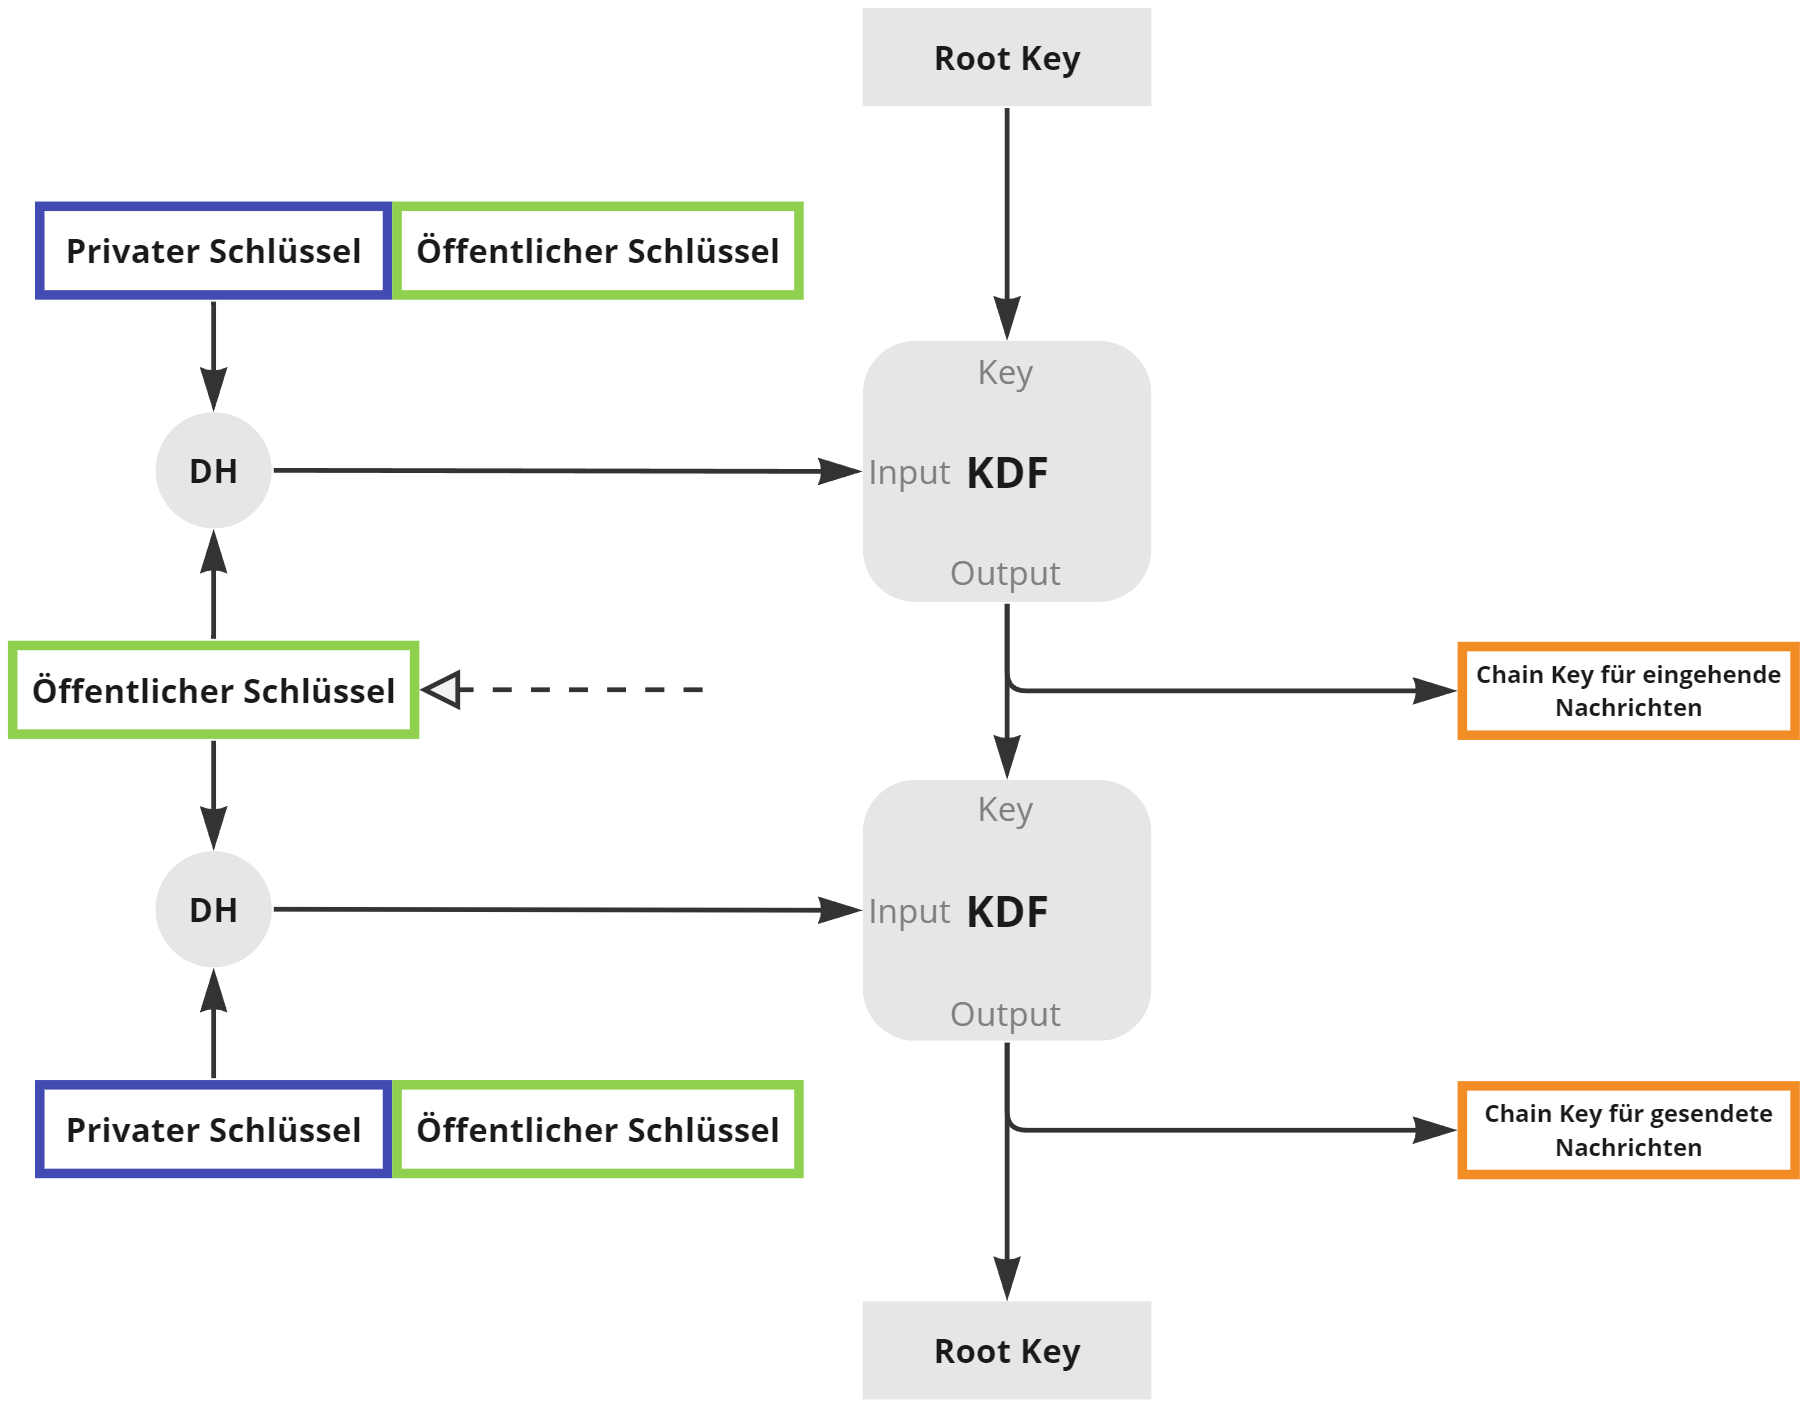
\includegraphics[width=0.8\linewidth]{images/double_ratchet_altered.png}
    \caption{Vereinfachter Double Ratchet Algorithmus (in Anlehnung an \cite{Signal_DoubleRatchet})}
    \label{fig:double_ratchet}
\end{center}

\noindent Links ist der zweite Ratchet-Schritt zu sehen (asymmetrischer Schlüsselaustausch). In der Abbildung ist dieser mit \textit{DH} gekennzeichnet, was für den Diffie-Hellman-Schlüsselaus-\\tausch steht. Auf der rechten Seite befindet sich der erste Ratchet-Schritt. Die Schlüsselableitungsfunktion wird in der Abbildung mit \textit{KDF} bezeichnet. Aus dieser werden die symmetrischen Schlüssel (in der Abbildung als \textit{Chain Key} bezeichnet) abgeleitet, die die jeweiligen Nachrichten ver- und entschlüsseln.





    %\chapter{Anforderungsanalyse}

% Lastenheft (auch Anforderungs- oder Kundespezifikation):
% - enthält eher abstrakte, eher allgemeine Festlegungen der gewünschten Dienste
% - fundamentale Eigenschaften des Produktes
% - Beschreibung des "was" und nicht des "wie"
% - hat den Sinn, der Lösung nicht vorzugreifen (Art der Umsetzung ist hier nicht relevant)

% Pflichtenheft:
% - Entwickler beschreibt wie er die im Lastenheft dargelegten Anforderungen zu erfüllen gedenkt
% - Beschreibung bis in das kleinste Detail, wie sich die Software unter bestimmten Bedingungen verhalten soll

Die Zielgruppe für dieses Protokoll sind Privatnutzer, woraus sich Anforderungen in den Bereichen Sicherheit,
Datenschutz und \dots


\section{Funktionale Anforderungen}


% Dies sind Aussagen zu den Diensten, die das System leisten sollte, zur Reaktion des Systems auf bestimmte 
% Eingaben und zum Verhalten des Systems in bestimmten Situationen. 

Funktionale Anforderungen beziehen sich auf die spezifischen Funktionen und Aufgaben, die eine Software oder ein System erfüllen muss, um die Bedürfnisse und Erwartungen der Benutzer zu erfüllen. Sie beschreiben, was das System tun soll, welche Aktionen es ausführen muss und welche Ergebnisse es liefern sollte. Mitunter werden sie auch dazu verwendet, um festzuhalten, was das System nicht können soll. All diese Anforderungen sind entscheidend, um sicherzustellen, dass die entwickelte Software oder wie in diesem Fall, das entwickelte Protokoll die erwarteten Funktionen erbringt. Sie dienen als Grundlage für das Design, die Entwicklung, die Validierung und die Verifizierung von Software-Systemen und sind ein wichtiger Bestandteil des Anforderungsmanagements im Software-Engineering-Prozess \parencite[S. 124-126]{Sommerville_AnfAnalyse}.

Um die Anforderungen an das zu entwickelnde Protokoll zu definieren, wird es in die folgenden
Funktionen unterteilt:

\begin{itemize}
    \item Peer-Discovery und Routing
    \item Verbindungsmanagement
    \item Nachrichtenformatierung
    \item Sicherheit und Verschlüsselung
    \item Plattformunabhängigkeit
    \item Fehlerbehandlung und Wiederholungsmechanismen
\end{itemize}

\noindent Die folgenden Abschnitte beschreiben die funktionalen Anforderungen an das Protokoll.

\subsection{Peer-Discovery und Routing}
\label{subsec:peer_discovery}

Das Protokoll muss es den Benutzern ermöglichen, sich gegenseitig zu finden, um miteinander kommunizieren zu können. Dazu muss es eine Möglichkeit geben, die IP-Adresse eines Benutzers zu ermitteln, wenn der Benutzername des Ziels bekannt ist. Wenn die IP-Adresse eines Benutzers bekannt ist, muss das Protokoll in der Lage sein, eine Verbindung zu diesem Benutzer herzustellen. Dies ist notwendig, um die Dezentralität des Protokolls zu gewährleisten. Sollte ein Art von zentralem Server benötigt werden, muss die Verschlüsselung der Nachrichten so implementiert werden, dass dem Server nicht vertraut werden muss und dieser damit nicht in der Lage ist, die Nachrichten zu entschlüsseln und zu lesen.
\subsection{Verbindungsmanagement}
\label{subsec:verbindungsmanagement_req}

Das Verbindungsmanagement in einem Peer-to-Peer Instant-Messaging-Protokoll umfasst verschiedene Aspekte, die für eine zuverlässige, stabile und sichere Kommunikation zwischen den Peers essentiell sind.

Zunächst spielt der Verbindungsaufbau eine wichtige Rolle. Dieser Mechanismus ermöglicht es den Peers, miteinander in Verbindung zu treten. Durch die Verwendung von IP-Adressen und Ports oder anderen Identifikationsmechanismen wird sichergestellt, dass die Kommunikation initiiert werden kann. Dieser Prozess sollte sicher und authentifiziert ablaufen, um die Integrität des Netzwerks zu gewährleisten. Die Überwachung der Verbindungsstabilität ist ein weiterer wichtiger Aspekt des Verbindungsmanagements. Durch regelmäßige Überprüfungen sollte sichergestellt werden, dass die Verbindung zwischen den Peers aktiv bleibt und eventuelle Probleme frühzeitig erkannt werden können. Ein weiterer Schlüsselaspekt ist die Verbindungsbeendigung. Ein ordnungsgemäßer Mechanismus zur Beendigung von Verbindungen ist wichtig, um Ressourcen freizugeben und mögliche Sicherheitsrisiken zu minimieren. Die Verbindungsbeendigung kann durch Benutzeraktionen wie das Abmelden ausgelöst werden oder aufgrund von Fehlern im Netzwerk auftreten. Im Falle vorübergehender Unterbrechungen, beispielsweise durch Netzwerkausfälle, sollte das Verbindungsmanagement Mechanismen zur automatischen Wiederherstellung von Verbindungen bereitstellen. Die Verbindungsauthentifizierung hingegen stellt sicher, dass die Kommunikation nur zwischen vertrauenswürdigen Parteien stattfindet. Dieser Sicherheitsaspekt ist entscheidend, um unautorisierte Zugriffe zu verhindern und die Vertraulichkeit der übertragenen Daten zu gewährleisten.
\subsection{Nachrichtenformatierung}

Die Nachrichtenformatierung ist ein wichtiger Aspekt eines Instant-Messaging-Protokolls. Sie definiert, wie die Nachrichten strukturiert sind und welche Informationen sie enthalten. Die Nachrichtenformatierung ist entscheidend für die Funktionalität des Protokolls, da sie die Grundlage für die Kommunikation zwischen den Peers bildet. Die Nachrichtenformatierung muss so gestaltet sein, dass sie die folgenden Anforderungen erfüllt:

\begin{itemize}
    \item Die Nachrichten müssen in einem standardisierten Format vorliegen, um die Interoperabilität zwischen den verschiedenen Implementierungen des Protokolls zu gewährleisten.
    \item Die Nachrichten müssen die erforderlichen Informationen enthalten, um die Kommunikation zwischen den Peers zu ermöglichen.
    \item Die Nachrichten müssen so strukturiert sein, dass sie von den Peers verarbeitet werden können.
\end{itemize}
\subsection{Verschlüsselung der Kommunikation}

% Wenn Public Key des anderen bekannt ist, gilt das als authentifizierter Schlüsselaustausch. Bietet Schutz 
% vor Man in the Middle Attacken, da bekannt ist, wem der Public Key gehört. Da in meinem Fall beide
% authentifiziert sind, ist es ein wechselseitiger authentifizierter Schlüsselaustausch.

Für die Verschlüsselung der Kommunikation soll das Public-Key-Verfahren verwendet werden.
Das Public-Key-Verfahren ist ein asymmetrisches Verschlüsselungsverfahren, das zwei Schlüssel verwendet,
einen öffentlichen und einen privaten Schlüssel. Das soll gewährleisten, dass die Nachrichten nur von
dem Benutzer gelesen werden können, für den sie bestimmt sind und erkannt werden kann, ob die Nachricht
manipuliert wurde. Zudem erhöht es die Sicherheit des Schlüsselaustauschs, da es praktisch unmöglich ist,
den privaten Schlüssel aus dem öffentlichen Schlüssel zu berechnen.


% Der öffentliche Schlüssel wird verwendet, um Nachrichten
% zu verschlüsseln, und der private Schlüssel wird verwendet, um Nachrichten zu entschlüsseln. Der öffentliche
% Schlüssel wird an alle Benutzer verteilt, während der private Schlüssel nur dem Benutzer bekannt ist.

%#TODO: DH bzw ECDH muss in den Grundlagen erklärt werden

% Für die Verschlüsselung wird der Elliptic Curve Diffie-Hellman-Schlüsselaustausch verwendet.
% Der Elliptic Curve Diffie-Hellman-Schlüsselaustausch ist ein Schlüsselaustauschprotokoll, das auf dem
% Diffie-Hellman-Schlüsselaustausch basiert. Der Diffie-Hellman-Schlüsselaustausch ist ein Schlüsselaustauschprotokoll,
% das verwendet wird, um einen gemeinsamen geheimen Schlüssel zwischen zwei Parteien zu erzeugen. Der
% gemeinsame geheime Schlüssel wird verwendet, um die Nachrichten zu verschlüsseln und zu entschlüsseln.
% Der Elliptic Curve Diffie-Hellman-Schlüsselaustausch verwendet elliptische Kurven, um die Sicherheit des
% Schlüsselaustauschs zu erhöhen. Die elliptische Kurve ist eine mathematische Funktion, die verwendet wird,
% um die Punkte zu berechnen, die für die Verschlüsselung und Entschlüsselung der Nachrichten verwendet werden.
% Der Elliptic Curve Diffie-Hellman-Schlüsselaustausch ist sicher, da es praktisch unmöglich ist, den
% gemeinsamen geheimen Schlüssel aus den öffentlichen Schlüsseln zu berechnen.
\subsection{Plattformunabhängigkeit}

Das Protokoll sollte auf verschiedenen Betriebssystemen und Gerätetypen nahtlos funktionieren. Um Plattformunabhängigkeit zu gewährleisten, sollte das Protokoll auf offenen, standardisierten Technologien basieren. Hierzu gehören beispielsweise Netzwerkprotokolle wie TCP, UDP oder IP. Die Verwendung plattformübergreifender Standards stellt sicher, dass die Kernfunktionalitäten des Protokolls von den meisten Betriebssystemen unterstützt werden. Die Implementierung der Protokollspezifikationen sollte in verschiedenen Programmiersprachen möglich sein. Dies ermöglicht es, das Protokoll in verschiedenen Anwendungen zu verwenden. Diese Unabhängigkeit ist ein wichtiger Aspekt, um die Verbreitung des Protokolls zu fördern und die Interoperabilität zwischen verschiedenen Anwendungen zu gewährleisten.
\subsection{Fehlerbehandlung und Wiederholungsmechanismen}

Die Fehlerbehandlung und die Implementierung von Wiederholungsmechanismen stellen entscheidende Komponenten im Verlauf einer Peer-to-Peer Instant-Messaging-Kommuni-\\kation dar. Ein zentraler Aspekt der Fehlerbehandlung ist die Erkennung von Übertragungsfehlern. Das Protokoll sollte in der Lage sein, Fehlerzustände während des Nachrichtenaustauschs zu identifizieren. Dies können beispielsweise fehlerhafte Pakete, verlorene Verbindungen oder andere unvorhergesehene Probleme sein. Die Fehlererkennung ermöglicht es, schnell auf Probleme zu reagieren und entsprechende Maßnahmen einzuleiten. Die Wiederholungsmechanismen sind eng mit der Fehlerbehandlung verbunden und dienen dazu, sicherzustellen, dass fehlgeschlagene Übertragungen erneut versucht werden. Dies könnte durch automatisches erneutes Senden von Nachrichten oder das Auslösen spezifischer Protokollmechanismen geschehen. Die Wiederholungsmechanismen sind darauf ausgerichtet, die Zustellung von Nachrichten trotz vorübergehender Probleme im Netzwerk zu gewährleisten.
 

%\subsection{Benutzeranforderungen und -erwartungen}

Benutzer erwarten die folgenden Funktionen...
%\subsection{Sicherheitsanforderungen an das Protokoll}

Sicherheitsanforderungen sind ...
\section{Nicht-funktionale Anforderungen}

%Dies sind Beschränkungen der durch das System angebotenen Dienste oder Funktionen. Das schließt 
%Zeitbeschränkungen, Beschränkungen des Entwicklungsprozesses und einzuhaltende Standards ein.

Nicht-funktionale Anforderungen sind Anforderungen, die sich nicht auf eine 
spezifische Funktionalität einer Software-Anwendung beziehen, sondern auf die Gesamtstruktur und damit auf
Qualitätsmerkmale und Aspekte, wie beispielsweise die Leistung, Zuverlässigkeit, Antwortzeit und Benutzerfreundlichkeit 
der Software. 
Diese Anforderungen beschreiben, \textit{wie} die Software funktionieren sollte, anstatt \textit{was} sie tun sollte. 
Nicht-funktionale Anforderungen sind genauso wichtig wie funktionale Anforderungen, da sie einen 
erheblichen Einfluss auf die Gesamtleistung und die Benutzerzufriedenheit haben können
\parencite[S. 126-130]{Sommerville_AnfAnalyse}.

\noindent Die folgenden nicht-funktionale Anforderungen soll das Protokoll bieten:

\begin{itemize}
    \item Performanz
    \item Sicherheit
    \item Zuverlässigkeit
    \item Kompatibilität
    %\item Interoperabilität
    \item Privatsphäre
    \item Skalierbarkeit
\end{itemize}

\noindent Die folgenden Abschnitte beschreiben die nicht-funktionalen Anforderungen an das Protokoll.

\subsection{Performanz}

Die Leistungsanforderungen an ein Peer-to-Peer Instant-Messaging-Protokoll beziehen sich auf die Effizienz und Geschwindigkeit der Nachrichtenübertragung, um sicherzustellen, dass Benutzer eine reaktionsschnelle und nahtlose Kommunikation erfahren. Die Leistungsfähigkeit des Protokolls beeinflusst direkt die Benutzerzufriedenheit und die Gesamterfahrung der Instant-Messaging-Anwendung, die das Protokoll verwendet. 



    \chapter{Architektur des Protokolls}
\label{chap:entwurf_und_architektur}

% #TODO: hashing in Betracht gezogen, aber da er nur dazu dient eine ID zu erzeugen bzw. man einen Nutzer daran identifizieren soll, ist das eigentlich nicht notwendig zu hashen. Es ist kryptografisch nicht notwendig
% #TODO: deshalb den Benutzernamen verwenden, der ja sowieso eindeutig sein muss (aus UX-Gründen), ihn auf 20 Zeichen limitieren (utf-8 -> 160 bits/8 = 20) und gegebenenfalls mit Nullen auffüllen, falls er kürzer ist

% #TODO: Vielleicht noch den Sicherheitsaspekt der Blockchain erklären, dass die IDs nicht gefälscht werden können, da sie in der Blockchain gespeichert sind und somit nicht manipuliert werden können; wenn die Nachrichten mit dem public key, der in der Blockchain liegt, signiert werden, bietet auch das eine Sicherheit, dass die Nachrichten nicht gefälscht werden können

% #TODO: neu schreiben, wenn der komplette Inhalt des Kapitels feststeht 
Die Architektur des Protokolls basiert auf Peer-to-Peer. Das bedeutet, dass alle Teilnehmer gleichberechtigt sind und es keinen zentralen Server gibt, der die Kommunikation steuert. Somit erfolgt die Kommunikation direkt zwischen den Teilnehmern. Alle Teilnehmer sind in einem Netzwerk organisiert, das aus verschiedenen Knoten besteht, wobei jeder Knoten einen Teilnehmer des Netzwerks repräsentiert. Die direkte Verbindung wird bevorzugt, erst wenn diese nicht möglich ist, wird die Nachricht über ein Relay weitergeleitet. Die Blockchain findet ihren Einsatz bei der Identifikation und Authentifizierung der Teilnehmer. Jeder Teilnehmer hat eine eindeutige ID, die aus dem Benutzernamen besteht und bei der Registrierung in der Blockchain gespeichert wird, und somit für alle Teilnehmer einsehbar ist. Somit kann jeder Teilnehmer einen anderen Teilnehmer anhand seiner ID identifizieren. Die Authentifizierung erfolgt ebenfalls über die Blockchain, indem der öffentliche Schlüssel des Teilnehmers in der Blockchain gesucht wird. Wenn der öffentliche Schlüssel gefunden wird und der Benutzername mit der ID übereinstimmt, ist der Teilnehmer authentifiziert. 

\section{Grundlagen des Protokolls}
\label{sec:grundlagen_des_protokolls}


Um die Peer-to-Peer Funktionalität für das Protokoll dieser Arbeit zu gewährleisten, wird ein mehrschichtiges Verfahren verwendet.

Für den effizienten Aufbau einer Direktverbindung zwischen zwei Teilnehmern kamen Chord und Kademlia in die engere Auswahl, welche beide lange Gegenstand intensiver Forschung waren, sowohl in der Industrie als auch in der akademischen Welt \parencite[S. 808]{MedranoChavez_ChordKademliaHighChurnScenarios}. 
Das Chord-Protokoll und das Kademlia-Protokoll sind zwei grundlegend verschiedene Ansätze zur Organisation von Peer-to-Peer-Netzwerken. Beide Protokolle sind strukturiert und bieten eine effiziente Ressourcenlokalisierung, aber sie unterscheiden sich in ihrer Routing-Struktur und der Art und Weise, wie sie die Knoteninformationen verwalten.

Chord basiert auf einer Ringstruktur (siehe Abbildung \ref{chord_ring}), bei der die Knoten in einem Ring angeordnet sind und jeder Knoten für einen bestimmten Schlüsselbereich verantwortlich ist. Die Verbindungen zwischen den Knoten sind durch ihren Platz im Ring definiert, wobei jeder Knoten eine Verbindung zu seinem nächsten Nachbarn im Uhrzeigersinn hat. Ein Knoten besitzt zwei Informationsmengen: eine \textit{Successor-Liste} und eine \textit{Finger-Tabelle}. Die Successor-Liste enthält die Knoten, die direkt nach dem Knoten im Uhrzeigersinn im Ring kommen. Die Anzahl der dort enthaltenen Knoten hängt davon ab, wie viele Knoten im Netzwerk insgesamt vorhanden sind. Die Finger-Tabelle enthält die Knoten, die für die Schlüsselbereiche verantwortlich sind, die durch eine Berechnung auf der ID des Knotens basieren \Parencite[S. 810-811]{MedranoChavez_ChordKademliaHighChurnScenarios}.

\begin{center}
    \captionsetup{type=figure}
    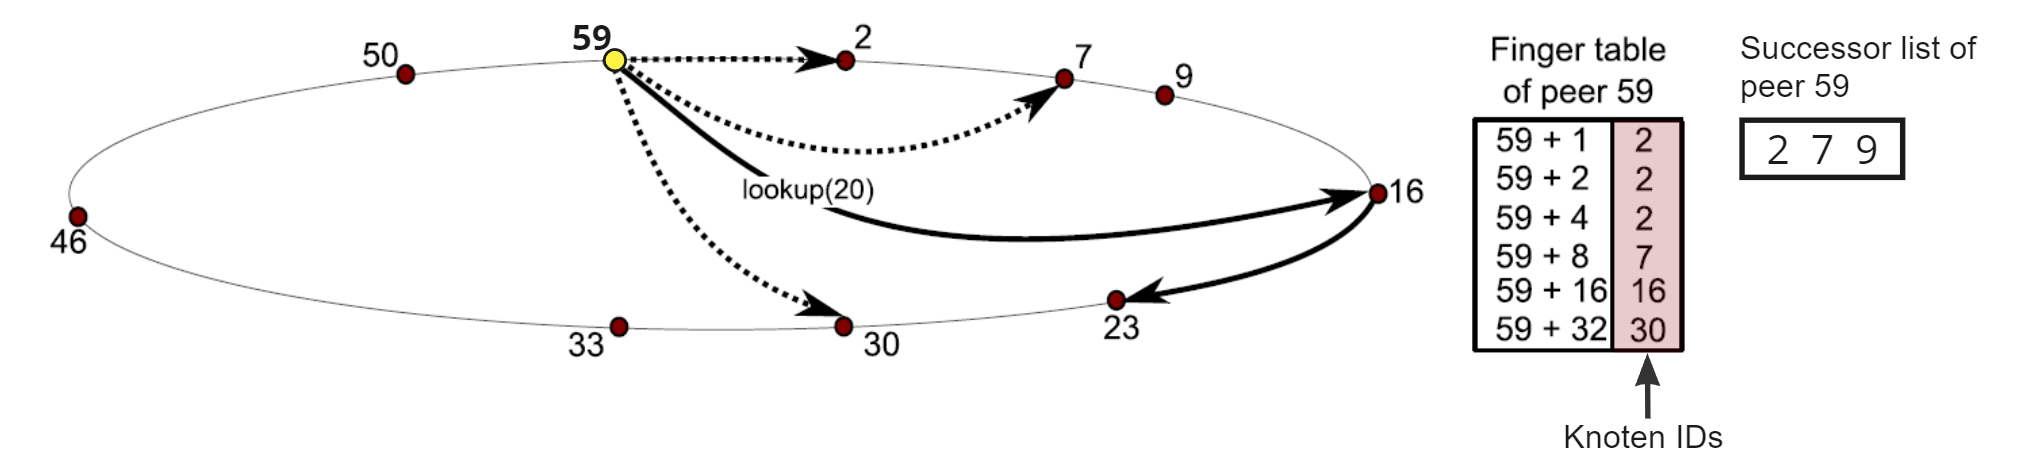
\includegraphics[width=1\linewidth]{images/chord_ring_altered.png}
    \captionof{figure}{Visualisierung der Ringstruktur von Chord, in Anlehnung an \cite[S. 811]{MedranoChavez_ChordKademliaHighChurnScenarios}}
    \label{chord_ring}
\end{center}

\noindent Wenn das Chord-Netzwerk eine Suchanfrage erhält, gibt es zwei Strategien, um die Anfrage zu bearbeiten. In der ersten Strategie wird die Anfrage sequentiell von Knoten zu Knoten weitergeleitet, bis der Knoten gefunden wird, der für den Schlüsselbereich verantwortlich ist, in dem sich der gesuchte Schlüssel befindet. Für diese Suchstrategie ergibt sich daher eine Komplexität von $\mathcal{O}(n)$, wobei $n$ die Anzahl der Knoten im Netzwerk ist. Die zweite Strategie verwendet die Finger-Tabelle, um die Anzahl der Knoten zu reduzieren, die die Anfrage weiterleiten. Diese Strategie hat eine Komplexität von $\mathcal{O}(\log n)$, wobei $n$ die Anzahl der Knoten im Netzwerk ist \parencite[S. 810-811]{MedranoChavez_ChordKademliaHighChurnScenarios}. 

In Abbildung \ref{chord_ring} ist zu erkennen, dass Knoten $59$ eine Suchanfrage für den Knoten mit der ID $20$ beginnt. Unter Verwendung der Finger-Tabelle von Knoten $59$ wird die Anfrage an den Knoten gesendet, der am nächsten an Knoten $20$ liegt. In diesem Fall ist dies Knoten $16$. Knoten $16$ wiederum leitet die Anfrage an den Knoten weiter, der ebenfalls am nächsten an Knoten $20$ liegt, was Knoten $23$ ist. Knoten $23$ ist für den Schlüsselbereich verantwortlich, in dem sich der gesuchte Schlüssel befindet, und sendet daher die Antwort an Knoten $59$ zurück. Durch die Verwendung dieser Strategie wurde Knoten $20$ in nur zwei Schritten gefunden, anstatt in fünft Schritten, wenn die Anfrage sequentiell weitergeleitet worden wäre.    

Im Gegensatz dazu verwendet Kademlia eine K-Bucket-Struktur, die in Abbildung \ref{kademlia_tree} zu sehen ist, um eine effiziente Verwaltung von Knoteninformationen zu ermöglichen. Die K-Buckets enthalten eine Liste von Knoten für verschiedene Schlüsselbereiche basierend auf ihrer Nähe, die durch XOR-Distanzen der IDs berechnet wird. Die Verbindungen zwischen den Knoten sind asymmetrisch, und jeder Knoten speichert Informationen über andere Knoten in seinen K-Buckets. Bei der Suche nach einem bestimmten Schlüssel erfolgt das Routing durch die XOR-Entfernung, wodurch die nächsten Knoten für diesen Schlüssel gefunden werden.

\begin{center}
    \captionsetup{type=figure}
    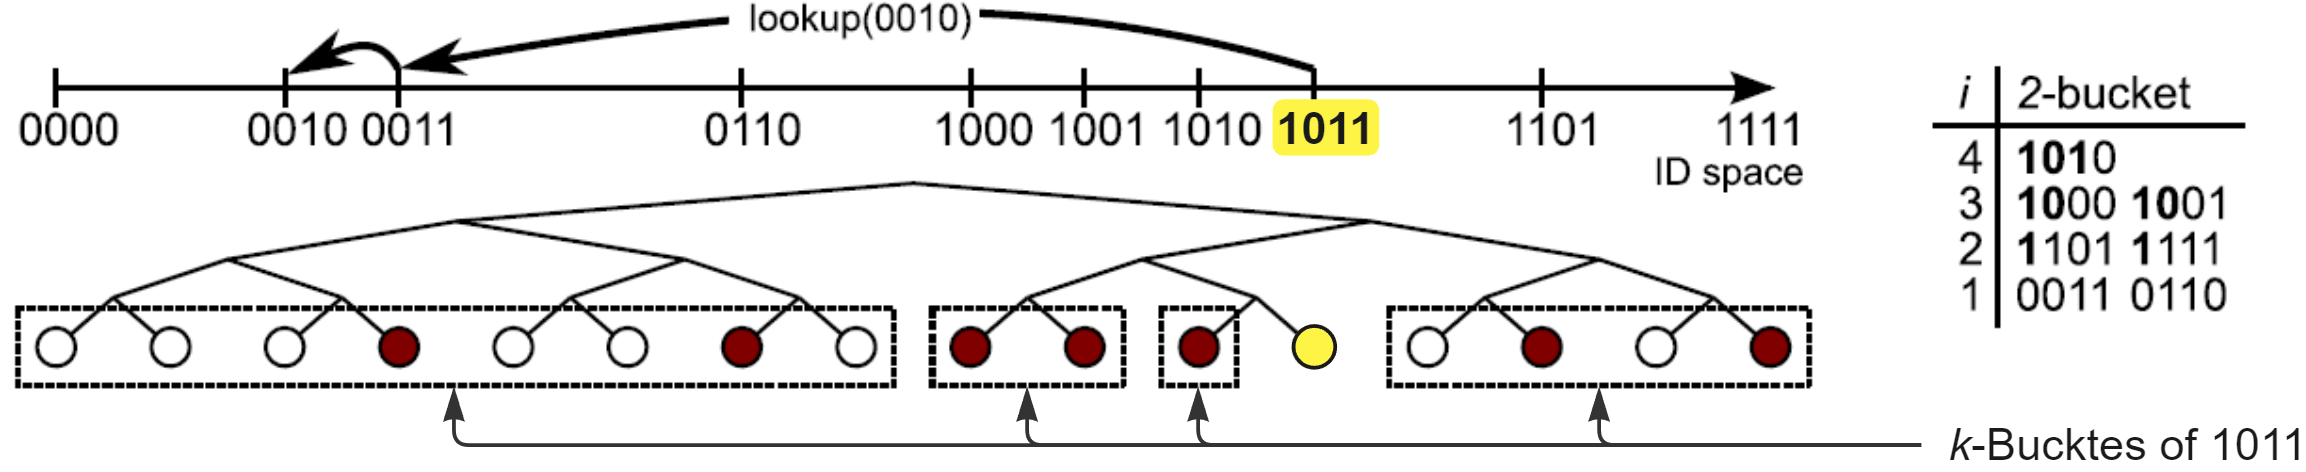
\includegraphics[width=1\linewidth]{images/kademlia_tree_altered.png}
    \captionof{figure}{Visualisierung der Baumstruktur von Kademlia, in Anlehnung an \cite[S. 812]{MedranoChavez_ChordKademliaHighChurnScenarios}}
    \label{kademlia_tree}
\end{center}

\noindent In Abbildung \ref{kademlia_tree} ist zu sehen, wie der Knoten $1011$ ein Suche nach Knoten $0010$ startet. Der Knoten $1011$ sucht in seinen vier K-Buckets nach dem nächsten Knoten, der am Schlüssel $0010$ liegt. Im ersten Bucket sind Knoten mit dem Präfix $0xxx$ enthalten. In Bucket zwei sind Knoten mit dem Präfix $11xx$, in Bucket drei Knoten mit dem Präfix $100x$ und in Bucket vier Knoten mit dem Präfix $101x$. Da der Schlüssel $0010$ mit dem Präfix $00$ beginnt, wird der nächste Knoten für diesen Schlüssel im ersten Bucket gesucht. Knoten $0011$ wird als nächster Knoten für den Schlüssel $0010$ gefunden. Knoten $1011$ sendet die Anfrage also an Knoten $0011$, der wiederum den nächsten Knoten für den Schlüssel $0010$ sucht. Da dieser Knoten den Schlüssel $0010$ in seinem K-Bucket besitzt, sendet er die Antwort auf die Suchanfrage an Knoten $1011$ zurück. Es werden zwei Weiterleitungen durchgeführt, um den Zielknoten zu finden, woraus sich eine Komplexität von $\mathcal{O}(\log n)$ ergibt, wobei $n$ die Anzahl der Knoten im Netzwerk ist \parencite[S. 812]{MedranoChavez_ChordKademliaHighChurnScenarios}.    


Da bei einem Instant-Messaging-Protokoll häufig Teilnehmer das Netzwerk verlassen und neue Teilnehmer dem Netzwerk beitreten, ist es wichtig, dass das Protokoll mit hoher Fluktuation umgehen kann. Diese Fluktuation von Nodes wird als Churn (engl. Abwanderung) bezeichnet. In einer Studie von Medrano-Chávez et al. \parencite{MedranoChavez_ChordKademliaHighChurnScenarios}, welche im hybriden Journal \textit{Peer-to-Peer Networking and Applications} veröffentlicht wurde, wurde die Leistung von Chord und Kademlia in Bezug auf Netzwerkfluktuation untersucht. Die Ergebnisse zeigen, dass Kademlia bei hoher Fluktuation besser abschneidet als Chord. Aus diesem Grund wird Kademlia in diesem Protokoll als Grundlage für das Auffinden von Teilnehmern und das Routing verwendet.

% #TODO: Warum Kademlia und was die Sicherheitsaspekte angeht, erst in Architektur aufgreifen.
    % Signaling Server könnte auch mit Anfragen geflutet werden -> der Sever könnte bei jedem checken, ob es sich um einen validen Teilnehmer handelt, was aber sehr aufwändig wäre
    % wenn Kademlia mit Anfragen geflutet wird, könnte es zu einem Denial of Service kommen, da die Knoten nicht mehr erreichbar sind -> habe aber ja mit dem Signaling Server noch eine weitere Instanz, die die Anfragen entgegen nimmt und weiterleitet


% #TODO: Overlay Netzwerk erklären? Kademlia ist ein Overlay Netzwerk
\begin{itemize}
    \item Kademlia vs. Angriffe
    \item Angriffe gegen ICE gucken und erklären
\end{itemize}

\noindent Um die Problematik mit NATs zu lösen, wird das ICE-Protokoll verwendet. ICE ist ein Framework, das mehrere Techniken kombiniert, um eine Verbindung zwischen zwei Endpunkten herzustellen, die sich hinter NATs befinden. Genaue Details zur Implementierung von ICE folgt in Kapitel \ref{subsec:verbindungsmanagement} \textit{\nameref{subsec:verbindungsmanagement}}.




\section{Identifikation von Teilnehmern}
\label{subsec:identifikation_von_teilnehmern}

Da es in Peer-to-Peer Netzwerken keinen zentralen Server gibt, der unter anderem zur Auffindung und Identifikation anderer Teilnehmer verwendet werden kann, müssen die Teilnehmer auf andere Weise identifiziert werden. Durch die Entscheidung, das Kademlia Protokoll zu implementieren, wird die ID des Teilnehmers als Schlüssel für die Speicherung der Teilnehmerinformationen, wie IP-Adresse und Port, verwendet.
Aus der Spezifikation von Kademlia geht hervor, dass die ID einer Node, welche auch als \textit{Kademlia-ID} bezeichnet wird, 160 Bit lang sein muss und aus einer zufälligen Kennung bestehen soll \parencite[S. 2]{Maymounkov_Kademlia}. Für das hier entwickelte Protokoll wird der Benutzername des Teilnehmers als ID verwendet. Dieser muss, wie aus den funktionalen Anforderungen zu entnehmen ist(siehe \ref{subsec:registrierung}), eindeutig sein und kann vom Benutzer bei der Registrierung frei gewählt werden. Um die Anforderung an die Länge zu erfüllen, werden die Zeichen des Benutzernamens auf 20 begrenzt und bei einer Formatierung in UTF-8 ergibt sich somit eine ID mit einer Länge von 160 Bit. Sollte der Benutzername kürzer als 20 Zeichen sein, wird er mit Nullen aufgefüllt, um die geforderte Länge zu erreichen.
Durch die Beschränkung der ID auf 20 Zeichen wird die Anzahl der möglichen Teilnehmer zwar begrenzt, doch daraus ergeben sich $2^{160}$ (65-stellige Zahl) mögliche IDs, was einer Anzahl von $1.461.501.637.330.902.918.203.684.832.716.283.019.655.932.542.976$ Teilnehmern entspricht. Diese Anzahl ist so groß, dass sie in der Praxis nicht erreicht werden sollte und somit die Beschränkung der ID keine Auswirkungen auf die Funktionalität des Protokolls haben sollte.

Wenn ein Teilnehmer eine Nachricht an einen anderen Teilnehmer senden möchte, muss er dessen IP-Adresse und Port kennen. Um an diese Informationen zu gelangen, muss zuerst die ID des Teilnehmers in der Blockchain gesucht werden und anschließend eine Peer-Discovery durchgeführt werden, um die IP-Adresse und den Port des Teilnehmers zu erhalten. Eine Peer-Discovery läuft wie folgt ab:

Dezentralisierte Netzwerke wie Kademlia verwenden Distributed Hash Tables (DHTs), um effizient Daten zu speichern und abzurufen. Im Kontext von Kademlia fungiert die DHT als Speichermechanismus für Informationen über die verfügbaren Teilnehmer im Netzwerk. Jede Node speichert normalerweise Informationen über andere Nodes in ihrer Nähe basierend auf ihrer Kademlia-ID und verwendet diese DHT, um schnell auf diese Daten zugreifen zu können. Die DHT ist in diesem Fall eine Routing-Tabelle, die die Teilnehmerinformationen enthält. Die Routing-Tabelle ist in Buckets aufgeteilt, wobei jeder Bucket eine bestimmte Distanz von der eigenen ID repräsentiert. Die Routing-Tabelle enthält 160 Buckets, wobei jeder Bucket eine Distanz von $2^{i}$ zu der eigenen ID repräsentiert, wobei $i$ die Nummer des Buckets ist. Jeder Bucket enthält eine Liste von Teilnehmern, die die Distanz des Buckets repräsentieren. Die Teilnehmer in einem Bucket sind nach der Zeit sortiert, in der sie zuletzt gesehen wurden, wobei der Teilnehmer, der zuletzt gesehen wurde, an erster Stelle steht. Die Routing-Tabelle wird verwendet, um die Teilnehmer zu finden, die eine bestimmte ID repräsentieren. Der Prozess beginnt mit der Berechnung der Distanz zwischen der eigenen ID und der ID des gesuchten Teilnehmers. Dazu wird die XOR-Operation auf den beiden IDs angewendet. Das Ergebnis ist eine 160 Bit lange Zahl, die die Distanz zwischen den beiden IDs repräsentiert. Diese Distanz wird nun in 160 Blöcke aufgeteilt, wobei jeder Block eine Bitlänge von 1 Bit hat. Die Blöcke werden von links nach rechts durchlaufen und die Bits werden von links nach rechts durchlaufen. Wenn ein Bit den Wert 1 hat, wird der Block in zwei Teile aufgeteilt und der Teil, der die ID des Teilnehmers repräsentiert, wird verwendet, um die nächste Node zu finden. Wenn ein Bit den Wert 0 hat, wird der Block nicht aufgeteilt und der Teil, der die eigene ID repräsentiert, wird verwendet, um die nächste Node zu finden. Dieser Vorgang wird solange wiederholt, bis die ID des Teilnehmers gefunden wurde. Wenn der Teilnehmer gefunden wurde, wird die IP-Adresse und der Port des Teilnehmers verwendet, um eine Verbindung zu ihm herzustellen.


\section{Nachrichtenformat}
\label{sec:nachrichtenformat}


Jedes Instant-Messaging-Protokoll benötigt die Definition eines Nachrichtenformats, das die Struktur der Nachrichten festlegt, die zwischen den Teilnehmern ausgetauscht werden. Im Folgenden wird das Nachrichtenformat für das Instant-Messaging-Protokoll beschrieben.
Nachdem eine Verbindung zwischen zwei Teilnehmern hergestellt werden konnte, kann die Nachricht vom Sender an den Empfänger gesendet werden. Die Nachricht wird in binär serialisierter Form übertragen und enthält die folgenden Informationen:

\begin{itemize}
    \item Benutzername des Senders
    \item Benutzername des Empfängers
    \item Timestamp
    \item Signatur
    \item Nachrichtenlänge
    \item Nachrichteninhalt
\end{itemize}

\noindent Bei der Erstellung des Nachrichtenformats wurde sich an \cite[S. 9]{rfc2779_IMPP} orientiert. Die Benutzernamen erlauben die Zuordnung der Nachricht. Der Timestamp enthält die aktuelle Zeit, zu der die Nachricht gesendet wird und wird für die richtige Sortierung der Nachrichten verwendet. Die Signatur dient der Authentifizierung des Senders (siehe \ref{subsec:vertrauliche_kommunikation} \textit{\nameref{subsec:vertrauliche_kommunikation}}). Aus Sicherheitsgründen wird jede Nachricht signiert. Die Nachrichtenlänge gibt die Länge des Nachrichteninhalts an und der Nachrichteninhalt enthält die eigentliche Nachricht, die vom Sender an den Empfänger gesendet werden soll.


\section{Verbindungsmanagement}
\label{subsec:routing}

\begin{itemize}
    \item Verbindungsaufbau (UDP)
    \item Nachrichtenübertragung
    \item Verbindungsabbau
\end{itemize}


\noindent Das Verbindungsmanagement ist ein wichtiger Bestandteil des Protokolldesigns, da es die Grundlage für die Kommunikation zwischen den Teilnehmern bildet. Es ist dafür verantwortlich, dass die Nachrichtenübertragung zwischen den Teilnehmern funktioniert. Dazu gehört der Verbindungsaufbau, die Nachrichtenübertragung und der Verbindungsabbau. In diesem Abschnitt wird der Verbindungsaufbau und der Verbindungsabbau behandelt.


Nach einer erfolgreichen Peer Discovery im Kademlia-Netzwerk, bei der die IP-Adresse und der Port des Zielknotens ermittelt wurde, erfolgt der Aufbau einer direkten Verbindung über das User Datagram Protocol (UDP). Dabei wird vorausgesetzt, dass bei allen Teilnehmern ein UDP-Socket an einem bestimmten Port geöffnet ist, um eingehende Verbindungen zu empfangen. Dieser Port wird vom Kademlia-Protokoll festgelegt und ist somit für alle Teilnehmer gleich.
Der Verbindungsaufbau erfolgt in folgenden Schritten:

\begin{enumerate}
    \item Der Sender erstellt ein UDP-Paket, das eine Verbindungsanfrage an den Empfänger enthält. Das Paket enthält die IP-Adresse und den Port des Senders, damit der Empfänger eine Antwort senden kann.
    \item Der Sender sendet das UDP-Paket an die IP-Adresse und den Port des Empfängers, welche er durch die Peer Discovery erhalten hat.
    \item Der Empfänger empfängt das UDP-Paket und überprüft, ob es sich um eine Verbindungsanfrage handelt.
    \item Der Empfänger sendet ein UDP-Paket als Antwort auf die Verbindungsanfrage an den Sender, die bestätigt, dass die Verbindung hergestellt wurde.
    \item Der Sender empfängt das UDP-Paket und überprüft, ob es sich um eine Bestätigung der Verbindungsanfrage handelt. Wenn dies der Fall ist, ist die Verbindung hergestellt und die Kommunikation kann beginnen. Wenn dies nicht der Fall ist, wird die Verbindung abgebrochen und der Verbindungsaufbau wird erneut gestartet.
\end{enumerate}

% #TODO: TURN-Server erklären und dessen IP-Adresse und Port in der Nachricht angeben, wenn die direkte Verbindung nicht möglich ist

\noindent Wie in Abschnitt \ref{subsec:identifikation_von_teilnehmern} (\nameref{subsec:identifikation_von_teilnehmern}) erwähnt, wird das Kademlia-Protokoll verwendet, um andere Teilnehmer (auch Peers genannt) im Netzwerk zu finden und eine direkte Verbindung zu ihnen herzustellen. \textcolor{red}{Begriff Peer Discovery einbringen}

% #TODO: Funktion des Kademlia Protokolls nennen und erklären (vielleicht in Grundlagen)
% Im Kademlia-Protokoll sind vier Funktionen definiert, die für die Suche nach
% Knoten und Werten verwendet werden. Diese Funktionen sind \texttt{FIND\_NODE},
% \texttt{FIND\_VALUE}, \texttt{PING} und \texttt{STORE}. Die Funktionen
% \texttt{FIND\_NODE} und \texttt{FIND\_VALUE} werden verwendet, um nach Knoten
% oder Werten zu suchen. Die Funktion \texttt{PING} wird verwendet, um die
% Erreichbarkeit eines Knotens zu überprüfen. Die Funktion \texttt{STORE} wird
% verwendet, um einen Wert in einem Knoten zu speichern.

%#TODO: Was wird jetzt für die ID verwendet? Benutzername oder Hashwert?
Das Kademlia-Protokoll basiert auf einem Distanzmetrik-Konzept, das als \enquote{Kademlia-Distanz} bekannt ist. Jeder Knoten im Netzwerk wird durch eine eindeutige ID repräsentiert, typischerweise als kryptografischer Hashwert, der sich in diesem Fall aus dem \textcolor{red}{gehashten?} öffentlichen Schlüssel des jeweiligen Knotens mittels der \textcolor{red}{SHA-1} Hashfunktion ergibt. Diese IDs sind in einem großen binären Baum organisiert, wobei die Position eines Knotens im Baum seine \enquote{Kademlia-Distanz} zu anderen Knoten definiert. Diese Distanz wird durch die XOR (ausschließendes Oder)-Operation ihrer eindeutigen IDs bestimmt. Die XOR-Operation ermöglicht eine effiziente Bestimmung der Distanz zwischen den Knoten-IDs, indem sie auf deren Binärzahlen angewendet wird. Dieses Ergebnis repräsentiert die Distanz zwischen den IDs und bildet die Grundlage für das Routing und die Organisation im Kademlia-Netzwerk.
Kademlia verwendet ein Routingverfahren, bei dem jeder Knoten eine Routing-Tabelle speichert, die als \enquote{K-Buckets} bezeichnet werden. Jedes K-Bucket enthält Verweise auf andere Knoten im Netzwerk und ist nach der Kademlia-Distanz organisiert. Ein k-Bucket enthält typischerweise eine begrenzte Anzahl von Einträgen und gruppiert Knoten mit ähnlichen IDs. 
Die Anzahl der Einträge in einem k-Bucket ist konfigurierbar und wird durch die Konstante \texttt{K} definiert. 
 \\
\textbf{Verbindungsaufbau} \\
Wenn ein Knoten eine Verbindung zu einem anderen Knoten herstellen muss, verwendet er die Routing-Tabelle, um den am nächsten gelegenen Knoten zu finden, der die Ziel-ID repräsentiert. Falls dieser Knoten nicht direkt bekannt ist, wird das Routing iterative durchgeführt, wobei der Knoten jeweils näher an der Ziel-ID liegende Knoten anfragt, bis der Zielknoten gefunden wird. Durch die Verwendung dieses strukturierten Ansatzes ermöglicht Kademlia eine effiziente Suche und Kommunikation zwischen Knoten in einem P2P-Netzwerk, wobei die Skalierbarkeit und Robustheit des Systems erhalten bleiben. Es ist ein Schlüsselelement vieler P2P-Anwendungen, einschließlich Filesharing, dezentraler Datenbanken und eben auch Instant Messaging-Protokollen, da es die Grundlage für die direkte Peer-to-Peer-Kommunikation schafft. Ein Beispiel für die XOR-Berechnung zwischen gehashten Knoten-IDs könnte wie folgt aussehen:
Angenommen, Knoten A hat die ID 0x83a2c8f7 und Knoten B die ID 0xe1b6d4a9.Die XOR-Operation zwischen diesen IDs ergibt:

\begin{equation}
    \begin{aligned}
        \text{Knoten A:} & \quad \texttt{0x83a2c8f7} \\
        \text{Knoten B:} & \quad \texttt{0xe1b6d4a9} \\
        \text{Ergebnis:} & \quad \texttt{0x61f47c5e}
    \end{aligned}
\end{equation}
% #TODO: Berechnung noch in binär umwandeln, damit die Berechnung besser verständlich ist?

\noindent Die Berechnung findet auf Bit-Ebene statt. Die Distanz zwischen den Knoten A und B ist also 0x61f47c5e. Diese Distanz repräsentiert die Maßeinheit für die Positionierung und das Routing im Kademlia-Netzwerk. Knoten mit einer geringeren Distanz sind näher beieinander als Knoten mit einer größeren Distanz. Dabei hat die Distanz nichts mit der geographischen Entfernung zu tun, sondern nur mit der Position im Kademlia-Baum.
\\

% #TODO: Zustellbestätigung?
% #TODO: ICE Protokoll verwenden, um die Verbindung aufzubauen, wenn die direkte Verbindung nicht möglich ist
% #TODO: Wie verbinde ich Kademlia und ICE? -> Kademlia für die Peer Discovery und ICE für den Verbindungsaufbau?

%\subsection{Status- und Präsenzinformationen}

Definieren Sie, wie Benutzer ihren Status aktualisieren (Online, Abwesend, Offline).
Überlegungen zur Präsenzinformation für effiziente Nachrichtenzustellung.

\subsection{Verbindungsmanagement}

Mechanismen für den Aufbau und die Beendigung von Peer-Verbindungen. Pufferung von Nachrichten für offline Benutzer.

Die Herstellung einer Verbindung zwischen zwei Teilnehmern ist ein wichtiger Aspekt eines Instant Messaging-Protokolls. Der Benutzer, der eine Verbindung aufbauen möchte, muss die eindeutige ID des anderen Benutzers kennen. DieseID wird verwendet, um eine Suche im Kademlia-Netzwerk durchzuführen, um den Knoten zu finden, der den Benutzer repräsentiert. Wenn der Knoten gefunden wurde, kann eine Verbindung hergestellt werden, indem eine Verbindungsanfrage gesendet wird. Wenn der Knoten die Anfrage akzeptiert, wird eine direkte Verbindung zwischen den beiden Knoten hergestellt. Wenn die Verbindung erfolgreich hergestellt wurde, können die Teilnehmer Nachrichten austauschen. Sollte der gesuchte Knoten nicht gefunden werden, wird auf ein TCP-Relay zurückgegriffen, um die Nachricht zu übermitteln. Dieses Relay ist ein Server, der die Nachrichten zwischen den Teilnehmern weiterleitet. Dieser Mechanismus wird verwendet, wenn die direkte Verbindung zwischen den Teilnehmern nicht möglich ist, z. B. wenn sich die Teilnehmer hinter einer Firewall befinden. Die Verwendung eines TCP-Relays ist jedoch nicht wünschenswert, da es die Skalierbarkeit des Systems beeinträchtigt und die Vertraulichkeit der Nachrichten gefährdet. Daher sollte die direkte Verbindung zwischen den Teilnehmern bevorzugt werden.


%\subsection{Verbindung und Identität}

Benutzer können andere Peers in einem verteilten Netzwerk entdecken und sich mit ihnen 
verbinden. Dies kann verteilte Hash-Tabellen (DHTs) oder andere Mechanismen zur 
Peer-Erkennung umfassen.
Benutzer werden durch eindeutige öffentliche Schlüssel identifiziert, und Benutzerprofile 
können zusätzliche Informationen wie Benutzernamen, Avatare und Status enthalten.

%\subsection{Nachrichten und Daten}

Benutzer können ausschließlich Textnachrichten miteinander austauschen. 
Diese Nachrichten können an einzelne Peers gesendet werden.
Die gesamte Kommunikation ist mit starken Verschlüsselungsalgorithmen 
verschlüsselt, um Privatsphäre und Sicherheit zu gewährleisten.

%\subsection{Nachrichtenverlauf}

Benutzer haben die Möglichkeit, ihren Nachrichtenverlauf lokal zu speichern.
Der Nachrichtenverlauf ist ebenfalls verschlüsselt, um die Sicherheit zu gewährleisten.

\section{Sicherheit}
\label{subsec:sicherheit}

% #TODO: Sessions könnten so ca. 10 Minuten dauern, dann wird ein neuer symmetrischer Schlüssel ausgehandelt
% Diffie-Hellman-Schlüsselaustausch basiert auf Gruppen, die aus einem Generator und einer Primzahl bestehen. Die Gruppen werden so gewählt, dass der diskrete Logarithmus in diesen Gruppen schwer zu berechnen ist. Der diskrete Logarithmus ist das inverse Element der Exponentialfunktion. Das bedeutet, dass der diskrete Logarithmus die Lösung der Gleichung $g^x = y$ ist, wobei $g$ der Generator, $x$ der diskrete Logarithmus und $y$ das Ergebnis der Exponentialfunktion ist. Die Schwierigkeit des diskreten Logarithmus ist, dass es keine effiziente Methode gibt, um ihn zu berechnen. Die Sicherheit des Diffie-Hellman-Schlüsselaustauschs basiert auf der Annahme, dass es keine effiziente Methode gibt, um den diskreten Logarithmus zu berechnen. Eine Gruppe kann aber auch aus einem elliptischen Kurvenpunkt und einer Primzahl bestehen. Die Sicherheit des Diffie-Hellman-Schlüsselaustauschs basiert auf der Annahme, dass es keine effiziente Methode gibt, um das diskrete Logarithmusproblem in elliptischen Kurven zu lösen.



\textcolor{red}{Quellenangaben, falls nicht schon in Grundlagen gemacht}


\noindent Um die Kommunikation zwischen den Teilnehmern zu schützen, wird sowohl asymmetrische als auch symmetrische Verschlüsselung verwendet. Die asymmetrische Verschlüsselung wird für die Authentifizierung und die symmetrische Verschlüsselung für die Ende-zu-Ende-Verschlüsselung der Nachrichten verwendet. Die asymmetrische Verschlüsselung wird mit Hilfe von Public-Key-Kryptographie realisiert. In dem von Whitfield Diffie und Martin Hellman 1976 veröffentlichten Paper \textit{New Directions in Cryptography} \parencite{DiffieHellman_NewDirectionsInCryptography} wurde die Public-Key-Kryptographie erstmals beschrieben. Darin wird die Problematik der symmetrischen Verschlüsselung beschrieben, dass ein Schlüssel für die Verschlüsselung und Entschlüsselung verwendet wird und dieser Schlüssel zu Beginn der Kommunikation über einen unsicheren Kanal  zwischen den Teilnehmern ausgetauscht werden muss. Die Lösung dieses Problems ist die Public-Key-Kryptographie.


Bei der Public-Key-Kryptographie wird ein Schlüsselpaar generiert, das aus einem öffentlichen und einem privaten Schlüssel besteht. In diesem Protokoll wird bei der Registrierung eines Teilnehmers ein statisches Schlüsselpaar generiert. Der öffentliche Schlüssel dieses Schlüsselpaars wird gemeinsam mit dem Benutzernamen in der Blockchain hinterlegt und der private Schlüssel wird lokal auf dem Gerät des Teilnehmers gespeichert.

Um die Ende-zu-Ende-Verschlüsselung zu realisieren, wird ein Diffie-Hellman Schlüsselaustausch durchgeführt, der auf elliptischen Kurven basiert und daher auch Elliptic-Curve-Diffie-Hellman-Schlüsselaustausch (oder kurz ECDH) genannt wird. Als Grundlage für einen Schlüsselaustausch muss sich auf eine gemeinsame elliptische Kurvengleichung geeinigt werden. Für das hier entwickelte Protokoll wird die Funktion \textit{X448} verwendet, die in RFC 7748 \textit{The X25519 and X448 Elliptic Curves} \parencite{rfc_ellipticCurves} spezifiziert ist.



Der Diffie-Hellman-Schlüsselaustausch basiert auf der Annahme, dass es keine effiziente Methode gibt, um den diskreten Logarithmus zu berechnen. Der Diffie-Hellman-Schlüsselaustausch basiert auf Gruppen, die aus einem Generator und einer Primzahl bestehen. Die Gruppen werden so gewählt, dass der diskrete Logarithmus in diesen Gruppen schwer zu berechnen ist. Der diskrete Logarithmus ist das inverse Element der Exponentialfunktion. Das bedeutet, dass der diskrete Logarithmus die Lösung der Gleichung $g^x = y$ ist, wobei $g$ der Generator, $x$ der diskrete Logarithmus und $y$ das Ergebnis der Exponentialfunktion ist. Die Schwierigkeit des diskreten Logarithmus ist, dass es keine effiziente Methode gibt, um ihn zu berechnen. Eine Gruppe kann aber auch aus einem elliptischen Kurvenpunkt und einer Primzahl bestehen. Die Sicherheit des Diffie-Hellman-Schlüsselaustauschs basiert auf der Annahme, dass es keine effiziente Methode gibt, um das diskrete Logarithmusproblem in elliptischen Kurven zu lösen.




Bei einem Verbindungsaufbau wird vom Sender ein neues Schlüsselpaar generiert, welches diesmal aus flüchtigen Schlüsseln besteht. Der Sender generiert einen flüchtigen privaten Schlüssel und einen flüchtigen öffentlichen Schlüssel. Der flüchtige öffentliche Schlüssel wird zusammen mit der ID des Senders und einem Zeitstempel in einer Nachricht, welche mit dem statischen privaten Schlüssel des Senders signiert wird, an den Empfänger gesendet. Der Empfänger kann die Nachricht mit dem öffentlichen Schlüssel des Senders, welcher mittels Smart Contract aus der Blockchain ausgelesen werden kann, entschlüsseln und somit die Authentizität des Senders verifizieren. Dadurch kann der Empfänger sicher sein, dass die Nachricht vom Sender stammt und nicht von einem Angreifer manipuliert wurde. Mit Hilfe des Zeitstempels kann der Empfänger außerdem feststellen, ob der flüchtige öffentliche Schlüssel noch gültig ist. Der Empfänger extrahiert den flüchtigen öffentlichen Schlüssel aus der Nachricht des Senders und ist somit im Besitz des flüchtigen öffentlichen Schlüssels des Senders. Der Empfänger generiert ebenfalls einen flüchtigen privaten Schlüssel und einen flüchtigen öffentlichen Schlüssel. Der flüchtige öffentliche Schlüssel wird zusammen mit der ID des Empfängers und einem Zeitstempel in einer Nachricht, welche mit dem statischen privaten Schlüssel des Empfängers signiert wird, an den Sender gesendet. Der Sender kann die Nachricht mit dem öffentlichen Schlüssel des Empfängers entschlüsseln und somit die Authentizität des Empfängers verifizieren. Nun sind beide Teilnehmer im Besitz des flüchtigen öffentlichen Schlüssels des jeweils anderen Teilnehmers.


Anschließend wird ein gemeinsamer geheimer Schlüssel aus dem flüchtigen privaten Schlüssel und dem öffentlichen Schlüssel des Empfängers mittels Key-Derivation-Funktion berechnet und die flüchtigen Schlüssel werden verworfen. Der berechnete flüchtige symmetrische Schlüssel wird für die Verschlüsselung der Nachrichten verwendet.

Durch die Anwendung von flüchtigen Schlüsseln wird die Sicherheit erhöht, da diese nur für eine kurze Zeit existieren und somit ein Angreifer nur für einen kurzen Zeitraum Zugriff auf diese hat. Mit Hilfe dieser Methode wird eine Ende-zu-Ende-Verschlüsselung ermöglicht, da nur der Sender und der Empfänger den gemeinsamen geheimen Schlüssel kennen. Selbst wenn die Verbindung über ein Relay läuft, kann dieses die Nachricht nicht entschlüsseln, da es den gemeinsamen geheimen Schlüssel nicht kennt. Die Verwendung von flüchtigen Schlüsseln hat jedoch auch Nachteile. So muss bei jedem Verbindungsaufbau ein neues Schlüsselpaar generiert werden, was einen erhöhten Rechenaufwand bedeutet. 



\section{Fehlerbehandlung}

Fehlerbehandlung und -vermeidung sind wichtige Aspekte eines Instant Messaging-Protokolls. Fehler können zu einer Unterbrechung der Verbindung zwischen den Teilnehmern führen. Um dies zu verhindern, werden verschiedene Mechanismen implementiert, die die Verbindung zwischen den Teilnehmern aufrechterhalten.

Netzwerkfehler können zu einer Unterbrechung der Verbindung zwischen den Teilnehmern führen. Um dies zu verhindern, wird eine Pufferung der Nachrichten implementiert. Wenn ein Teilnehmer eine Nachricht sendet, wird diese in einem Puffer gespeichert, bis der Empfänger die Nachricht empfangen hat. Wenn der Empfänger die Nachricht nicht empfangen kann, wird sie im Puffer gespeichert, bis der Empfänger wieder online ist. Wenn der Empfänger wieder online ist, wird die Nachricht erneut gesendet. Wenn der Empfänger die Nachricht empfangen hat, wird sie aus dem Puffer gelöscht. Wenn der Empfänger die Nachricht nicht empfangen kann, wird sie nach einer bestimmten Zeit aus dem Puffer gelöscht. Die Pufferung der Nachrichten ermöglicht es, die Verbindung zwischen den Teilnehmern aufrechtzuerhalten, auch wenn einer der Teilnehmer offline ist. Dies ist ein wichtiger Aspekt für ein Instant Messaging-Protokoll, da die Teilnehmer nicht immer online sind. 
\\
\\
Firewall und NAT können ebenfalls zu Verbindungsproblemen führen. Um dies zu verhindern, wird ein TCP-Relay verwendet, um die Nachrichten zwischen den Teilnehmern weiterzuleiten. Dieser Mechanismus wird verwendet, wenn die direkte Verbindung zwischen den Teilnehmern nicht möglich ist, z. B. wenn sich die Teilnehmer hinter einer Firewall befinden. Die Verwendung eines TCP-Relays ist jedoch nicht wünschenswert, da es die Skalierbarkeit des Systems beeinträchtigt und die Vertraulichkeit der Nachrichten gefährdet. Daher sollte die direkte Verbindung zwischen den Teilnehmern bevorzugt werden.
\\
\\
Peer-spezifische Fehler:
\\
\\
In einem Peer-to-Peer-Netzwerk kann es häufig vorkommen, dass der gewünschte Teilnehmer nicht online und somit nicht Teil des Netzwerks ist. In diesem Fall wird eine Fehlermeldung an den Absender zurückgegeben, dass der gewünschte Teilnehmer nicht gefunden werden konnte. Wie diese Fehlermeldung implementiert wird, ist dem Entwickler überlassen. Ein weiterer Fehler könnte im Zusammenhang mit Authentifizierung entstehen. Wenn ein Teilnehmer eine Nachricht an einen anderen Teilnehmer senden möchte, muss er sich zuerst authentifizieren. Die Authentifizierung erfolgt über die Blockchain, indem der öffentliche Schlüssel des Teilnehmers mit der ID des Teilnehmers verglichen wird. Wenn die IDs übereinstimmen, ist der Teilnehmer authentifiziert und die Nachricht kann gesendet werden. Wenn die IDs nicht übereinstimmen, ist der Teilnehmer nicht authentifiziert und die Nachricht wird nicht gesendet. In diesem Fall wird eine Fehlermeldung an den Absender zurückgegeben, dass der Teilnehmer nicht authentifiziert ist. Wie diese Fehlermeldung implementiert wird, ist dem Entwickler überlassen.
\\
\\
Nachrichtenbezogene Fehler:
\\
\\
Es besteht die Möglichkeit, dass Teile von Nachrichten oder auch ganze Nachrichten verloren gehen können. Da Kademlia über UDP läuft, hat es nicht die Möglichkeiten, die beispielsweise TCP bietet. TCP kann bei Paketverlust die Pakete erneut senden, UDP kann dies nicht. Zusätzlich können Nachrichten beschädigt werden (\textcolor{red}{Prüfsumme?}).

\section{Protokollstruktur}
\label{sec:protokolldesign_und_struktur}

% Das Protokoll basiert auf Peer-to-Peer. Die direkte Verbindung mittels DHTs wird
% bevorzugt, erst wenn diese nicht möglich ist, wird die Nachricht über ein TCP-Relay
% weitergeleitet.




\section{Technologien und Tools}
Für die Umsetzung dieses Designs wurden diese Technologien verwendet.

\section{Integration von Blockchain}
\label{sec:blockchainintegration}


\subsection{Auswahl der Blockchain}
Für die Integration der Blockchain in das Protokoll wurde zunächst eine geeignete Blockchain gesucht. Dabei wurde sich auf die beiden bekanntesten Blockchains, Bitcoin und Ethereum, beschränkt. Da Bitcoin eine reine Kryptowährung ist und keine Smart Contracts unterstützt, wurde sich für Ethereum entschieden. Ethereum ist eine Blockchain, die zwar auch eine Kryptowährung, Ether, besitzt, aber zusätzlich auch Smart Contracts unterstützt. Der Grund für die Existenz einer Währung auf der Blockchain ist, dass die Smart Contracts, die auf der Blockchain ausgeführt werden, mit Ether bezahlt werden müssen \parencite[S. 2]{Antonopoulos_MasteringEthereum}. Somit ist es nicht möglich, Smart Contracts auf der Blockchain auszuführen, ohne Ether zu besitzen. Da die Smart Contracts auf der Blockchain aber mit Ether bezahlt werden müssen, ist es notwendig, dass jeder Nutzer, der einen Smart Contract ausführen möchte, Ether besitzt.


\subsection{Registrierung}
Um das Protokoll zu nutzen, muss sich jeder Nutzer zunächst auf der Blockchain registrieren. Dazu muss ein Smart Contract auf der Blockchain ausgeführt werden, der die Registrierung des Nutzers durchführt. Dieser Smart Contract wird mit dem Benutzernamen und dem statischen öffentlichen Schlüssel aufgerufen. Der statische öffentliche Schlüssel wird bei der Registrierung festgelegt und kann nicht mehr geändert werden. Der Smart Contract erstellt einen neuen Eintrag in der Blockchain, der den Benutzernamen und den öffentlichen Schlüssel des Nutzers enthält. Der Smart Contract wird nur einmalig bei der Registrierung aufgerufen. Sollte ein Nutzer seinen Benutzernamen ändern wollen, muss er sich mit dem neuen Benutzernamen und dem öffentlichen Schlüssel eines neu erzeugten statischen Schlüsselpaars erneut registrieren.
% Der alte Benutzername wird dann aus der Blockchain gelöscht. -> wie könnte man das absichern?

\subsection{Kommunikation}
Für die Kommunikation mit anderen Teilnehmern, muss zunächst die ID des anderen Teilnehmers im Kademlia-Netzwerk bekannt sein. Dazu wird der Benutzername des anderen Teilnehmers auf der Blockchain gesucht um zu kontrollieren, ob dieser bereits registriert ist. Ist der Benutzername nicht auf der Blockchain vorhanden, ist der andere Teilnehmer nicht registriert und es kann keine Verbindung aufgebaut werden. Ist der Benutzername auf der Blockchain vorhanden, wird der dazugehörige öffentliche Schlüssel ausgelesen. Der Benutzername entspricht gleichzeitig der ID des Teilnehmers im Kademlia-Netzwerk. Somit kann der Verbindungsaufbau, der in Abschnitt \ref{subsec:verbindungsmanagement} \nameref{subsec:verbindungsmanagement} beschrieben wird, durchgeführt werden.
Wenn der Verbindungsaufbau erfolgreich war, kann die Kommunikation beginnen. Dazu wird der öffentliche Schlüssel des anderen Teilnehmers benötigt. Dieser wird ebenfalls auf der Blockchain gespeichert. Somit kann jeder Teilnehmer die öffentlichen Schlüssel der anderen Teilnehmer auf der Blockchain finden und die Nachrichten, die er erhält, mit dem öffentlichen Schlüssel des Absenders verifizieren. Somit kann sichergestellt werden, dass die Nachrichten tatsächlich vom angegebenen Absender stammen und nicht von einem anderen Teilnehmer gesendet wurden, der sich als jemand anderes ausgibt.

\subsection{Entwurf der Smart Contracts}
\label{subsec:smartcontracts}

Auf der Ethereum-Blockchain wird die hauptsächlich Programmiersprache Solidity verwendet, um Smart Contracts zu erstellen. Solidity ist eine objektorientierte Programmiersprache, die stark an JavaScript angelehnt ist \parencite[S. 131]{Antonopoulos_MasteringEthereum}. Die Smart Contracts, die für das Protokoll benötigt werden, sind in Solidity implementiert.




% Grundlegende Schritte und Überlegungen für das Protokolldesign:

% 1. **Identifikation von Teilnehmern:**
%    - Jeder Benutzer im Netzwerk hat eine eindeutige ID.
%    - Adressierung kann über Benutzer-IDs oder Schlüsselpaare erfolgen.

% 2. **Nachrichtenformat:**
%    - Struktur für Nachrichten festlegen (Header, Body, etc.).
%    - Verschlüsselung und Authentifizierung für Sicherheit hinzufügen.

% 3. **Routing und Weiterleitung:**
%    - Festlegen, wie Nachrichten im Netzwerk weitergeleitet werden (z.B., DHT basiert).
%    - Adressauflösung für direkte Peer-Kommunikation.

% 4. **Status- und Präsenzinformationen:**
%    - Definieren Sie, wie Benutzer ihren Status aktualisieren (Online, Abwesend, Offline).
%    - Überlegungen zur Präsenzinformation für effiziente Nachrichtenzustellung.

% 5. **Verbindungsmanagement:**
%    - Mechanismen für den Aufbau und die Beendigung von Peer-Verbindungen.
%    - Pufferung von Nachrichten für offline Benutzer.

% 6. **Gruppenkommunikation:**
%    - Implementierung von Gruppenchats oder Broadcast-Möglichkeiten.
%    - Berücksichtigung von Datenschutz und Berechtigungen.

% 7. **Sicherheit:**
%    - Integration von Verschlüsselung für Datenschutz und Sicherheit.
%    - Schutz vor Angriffen wie Man-in-the-Middle.

% 8. **Fehlerbehandlung:**
%    - Definition von Fehlercodes und deren Behandlung.
%    - Wiederholungsmechanismen für verlorene oder fehlerhafte Nachrichten.

% 9. **Benachrichtigungen:**
%    - Mechanismen für Benachrichtigungen über neue Nachrichten oder Statusänderungen.

% 10. **Protokollversionierung:**
%     - Implementierung von Versionierung für zukünftige Aktualisierungen.

    %\chapter{Evaluierung}

Hier ist die Evaluierung.
    %\chapter{Diskussion}

Hier ist die Diskussion.
    %\chapter{Schlussfolgerung und Ausblick}

Hier ist die Schlussfolgerung.
    %%%%%%%%%%%%%%%%%%%%%%%%%%%%%%%%%%%%% END: Numbered Chapters %%%%%%%%%%%%%%%%%%%%%%%%%%%%%%%%%%%%


    %%%%%%%%%%%%%%%%%%%%%%%%%%%%%%%%%%%%% BEGIN: Literature %%%%%%%%%%%%%%%%%%%%%%%%%%%%%%%%%%%%%%%%%
    \printbibliography[nottype=online]
    %\printbibliography[nottype=online, title={Standards}]
    %\printbibliography[nottype=online, title={Papers}]
    \printbibliography[type=online, title={Webseiten}]
    %%%%%%%%%%%%%%%%%%%%%%%%%%%%%%%%%%%%% END: Literature %%%%%%%%%%%%%%%%%%%%%%%%%%%%%%%%%%%%%%%%%%%

\end{document}